\PassOptionsToPackage{usenames,dvipsnames}{xcolor}
\documentclass[a4paper,12pt]{letter}
\usepackage[utf8]{inputenc}
\usepackage[T1]{fontenc}
\usepackage[english,slovene]{babel}
\usepackage[tikz]{bclogo}
\usepackage{marvosym}
\usepackage{tikz}
\usepackage{mathrsfs}
\usetikzlibrary{arrows,angles,quotes}
\usepackage{graphicx}
\newcommand{\ds}{\displaystyle}
\usepackage{fancybox}
\usepackage{amsfonts}
\usepackage{amsmath}
\usepackage{wallpaper}
\usepackage{hyperref}
\usepackage{array}
\newcolumntype{M}[1]{>{\centering\arraybackslash}m{#1}}
\newcolumntype{N}{@{}m{0pt}@{}}
\usepackage{fancyhdr,enumerate}
\newcommand{\ora}{\overrightarrow}
\renewcommand{\headrulewidth}{3pt}
\renewcommand{\headrule}{\hbox to\headwidth{%
  \color{gray}\leaders\hrule height \headrulewidth\hfill}}
\renewcommand{\footrulewidth}{2pt}
\renewcommand{\footrule}{\hbox to\headwidth{%
  \color{brown}\leaders\hrule height \footrulewidth\hfill}}
\usepackage{gensymb}
\usepackage{amssymb}
  \textwidth 20 true cm
  \oddsidemargin -2 true cm
  \evensidemargin -2 true cm
  \topmargin -3.5 true cm
  \textheight 27.5 true cm
  \linespread{1.2}
\renewcommand{\headrulewidth}{0.3pt}
\renewcommand{\footrulewidth}{1.9pt}
\definecolor{qqwuqq}{rgb}{1,0,0}
\definecolor{qqqqff}{rgb}{0,0,1}
\definecolor{qqffqq}{rgb}{0,1,0}
\definecolor{ffqqqq}{rgb}{1,0,0}
\definecolor{zzuxux}{rgb}{0,0,0}
\usepackage{mdframed}
\usepackage{multicol}
\definecolor{bgblue}{RGB}{0,0,253}
\usepackage{eurosym}
%%%%%%%%%%%%%%%%%%%%%%%%%%%%%%%%%%%%%%%%%%%%%%%%%%%%%%%%
\newcounter{tocke}
\setcounter{tocke}{0}
%%%%%%%%%%%%%%%%%%%%%%%%%%%%%%%%%%%%%%%%%%%%%%%%%%%%%%%%%%
\mdfdefinestyle{theoremstyle}{%
linecolor=brown!40,linewidth=1pt,%
frametitlerule=true,%
frametitlebackgroundcolor=brown!50,
innertopmargin=\topskip,
}
\mdfdefinestyle{theoremstyle1}{%
linecolor=brown,middlelinewidth=1pt,%
frametitlerule=true,%
apptotikzsetting={\tikzset{mdfframetitlebackground/.append style={%
shade,left color=black!40, right color=gray!10},
mdfbackground/.append style={
top color=white!100!white,
bottom color=black!5
},
}},
frametitlerulecolor=gray,
frametitlerulewidth=2pt,
innertopmargin=\topskip,
innerbottommargin=\topskip,
}
\mdtheorem[style=theoremstyle1]{naloga}{Naloga}
\mdtheorem[style=theoremstyle]{resitev}{Analiza Naloge}
\mdtheorem[style=theoremstyle]{kriterij}{\v{S}tevilo dose\v{z}enih to\v{c}k na testu}
%%%%%%%%%%%%%%%%%%%%%%%%%%%%%%%%%%%%%%%%%%%%%%%%%%%%%%%%%%
\usepackage[table]{xcolor}
\usepackage[angle=45,scale=5,color=brown!8,text={matej.info}]{draftwatermark}
%%%%%%%%%%%%%%%%%%%%%%%%%%%%%%%%%%%%%%%%%%%%%%%%%%%%%%%%%%

\begin{document}
\pagestyle{fancy}
\renewcommand\headrulewidth{0pt}
\lhead{}\chead{}\rhead{}
\rfoot{\vspace*{-2\baselineskip}}
\renewcommand{\vec}{\overrightarrow}
%%%%%%%%%%%%%%%%%%%% podatki testa -- tu spreminjaj
\def\programletnik{G-3}
\def\naslov{Naloge - }
\def\sklop{Kotne funkcije  - 3.del}
%%%%%%%%%%%%%%%%%%%% tocke po nalogah
\def\tockeA{16}
\def\tockeB{20}
\def\tockeC{4}
\def\tockeD{4}
\def\tockeE{6}
\def\tockeF{6}
\def\tockeG{12}
%%%%%%%%%%%%%%%%%%%%
\begin{minipage}{20cm}
\begin{bclogo}[couleur=brown!30,
  arrondi=0,ombre=true, couleurOmbre=gray!50,
logo =\bcplume,
  noborder=true]
{\textrm{{\Large{\naslov \sklop} \Huge{}
\large{} \hfill $\programletnik$}}}
\end{bclogo}
\end{minipage}
\begin{minipage}{20cm}
\begin{bclogo}[couleur=brown!30,
  arrondi=0,ombre=true, couleurOmbre=gray!50,
logo =\bcplume,
  noborder=true]
{\textrm{{\raisebox{-0.3cm}{\large{Ime in Priimek: \rule{10cm}{0.1mm}} \Huge{}
\large{} \hfill $ $}}}}
\end{bclogo}
\end{minipage}

\begin{naloga}[\hfill $\tockeA$] \addtocounter{tocke}{\numexpr\tockeA\relax}
Adicijski izreki, faktorizacija in defaktorizacija -- zahtevnej\v{s}e naloge.
\begin{enumerate}[a)]
\item Poenostavi izraz: $\displaystyle \frac{(\sin3x-\sin2x)\cos\frac{x}{2}}{\cos\frac{5x}{2}}$
\item Doka\v{z}i: $\displaystyle 4\sin33\degree\sin27\degree\cos3\degree=\cos9\degree$
\item Doka\v{z}i: $\displaystyle \sin20\degree\sin40\degree\sin80\degree=\frac{\sqrt3}{8}$
\item Izra\v{c}unaj brez kalkulatorja: $\displaystyle \cos20\degree\cos40\degree\cos80\degree$ \quad (namig: pomno\v{z}i in deli z $\sin20\degree$)
\item Poenostavi izraz: $\displaystyle \frac{\sin x+\sin3x+\sin5x}{\cos x+\cos3x+\cos5x}$
\item Doka\v{z}i: $\displaystyle \frac{\cos x-\cos3x}{\sin3x-\sin x}=\tan2x$
\item Izra\v{c}unaj brez kalkulatorja: $\displaystyle \cos^273\degree+\cos^247\degree+\cos73\degree\cos47\degree$
\item Doka\v{z}i: \v{c}e je $\alpha+\beta=45\degree$, potem je $(1+\tan\alpha)(1+\tan\beta)=2$.
\end{enumerate}
\end{naloga}
\begin{naloga}[\hfill $\tockeB$] \addtocounter{tocke}{\numexpr\tockeB\relax}
Nari\v{s}i graf funkcije s pomo\v{c}jo transformacij osnovnega grafa $y=\sin x$ oziroma $y=\cos x$ (premiki, raztegi, zrcaljenja). Vsak vmesni korak nari\v{s}i v isti koordinatni sistem. Zapi\v{s}i zalogo vrednosti $Z_f$ in osnovno periodo $\omega$.
\begin{enumerate}[a)]
\item $\displaystyle f(x)=\sin\Big(x+\frac{\pi}{4}\Big)$
\begin{center}
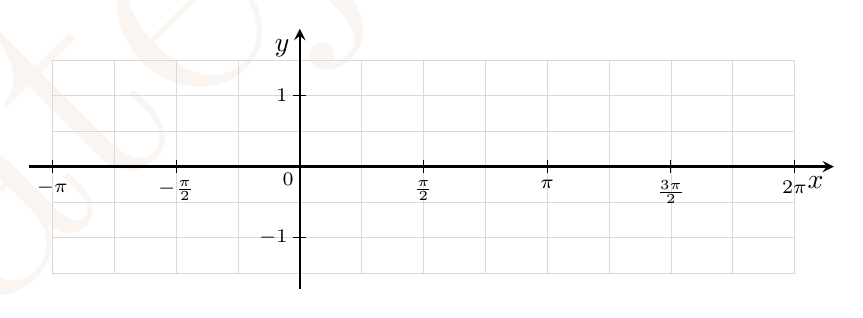
\begin{tikzpicture}[xscale=1,yscale=0.9,>=stealth]
\draw[very thin,gray!30,xstep=0.785398,ystep=0.5] (-3.1416,-1.5) grid (6.2832,1.5);
\draw[->,thick] (-3.4416,0) -- (6.7832,0) node[below left] {$x$};
\draw[->,thick] (0,-1.72222) -- (0,1.94444) node[below left] {$y$};
\draw (-3.1416,0.0889) -- (-3.1416,-0.0889);
\node[below,inner sep=2pt] at (-3.1416,-0.1111) {\scriptsize $-\pi$};
\draw (-1.5708,0.0889) -- (-1.5708,-0.0889);
\node[below,inner sep=2pt] at (-1.5708,-0.1111) {\scriptsize $-\tfrac{\pi}{2}$};
\draw (1.5708,0.0889) -- (1.5708,-0.0889);
\node[below,inner sep=2pt] at (1.5708,-0.1111) {\scriptsize $\tfrac{\pi}{2}$};
\draw (3.1416,0.0889) -- (3.1416,-0.0889);
\node[below,inner sep=2pt] at (3.1416,-0.1111) {\scriptsize $\pi$};
\draw (4.7124,0.0889) -- (4.7124,-0.0889);
\node[below,inner sep=2pt] at (4.7124,-0.1111) {\scriptsize $\tfrac{3\pi}{2}$};
\draw (6.2832,0.0889) -- (6.2832,-0.0889);
\node[below,inner sep=2pt] at (6.2832,-0.1111) {\scriptsize $2\pi$};
\draw (0.0800,-1) -- (-0.0800,-1) node[left,inner sep=2pt] {\scriptsize $-1$};
\draw (0.0800,1) -- (-0.0800,1) node[left,inner sep=2pt] {\scriptsize $1$};
\node[below left,inner sep=2pt] at (0,0) {\scriptsize $0$};
\end{tikzpicture}
\end{center}
\begin{center}$Z_f=$\,\rule{4cm}{0.1mm}\qquad $\omega=$\,\rule{3cm}{0.1mm}\end{center}

\item $\displaystyle f(x)=\cos\Big(x-\frac{\pi}{3}\Big)$
\begin{center}
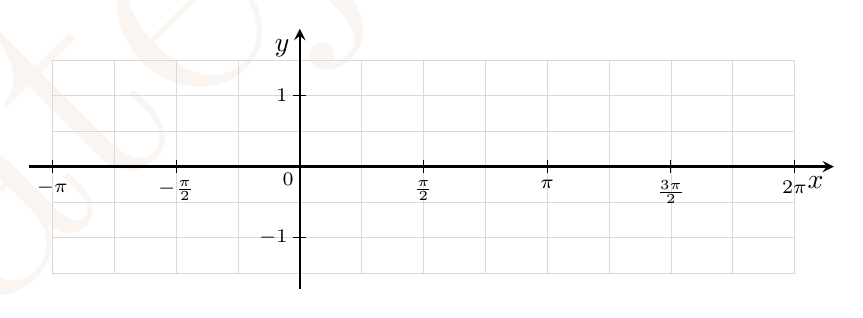
\begin{tikzpicture}[xscale=1,yscale=0.9,>=stealth]
\draw[very thin,gray!30,xstep=0.785398,ystep=0.5] (-3.1416,-1.5) grid (6.2832,1.5);
\draw[->,thick] (-3.4416,0) -- (6.7832,0) node[below left] {$x$};
\draw[->,thick] (0,-1.72222) -- (0,1.94444) node[below left] {$y$};
\draw (-3.1416,0.0889) -- (-3.1416,-0.0889);
\node[below,inner sep=2pt] at (-3.1416,-0.1111) {\scriptsize $-\pi$};
\draw (-1.5708,0.0889) -- (-1.5708,-0.0889);
\node[below,inner sep=2pt] at (-1.5708,-0.1111) {\scriptsize $-\tfrac{\pi}{2}$};
\draw (1.5708,0.0889) -- (1.5708,-0.0889);
\node[below,inner sep=2pt] at (1.5708,-0.1111) {\scriptsize $\tfrac{\pi}{2}$};
\draw (3.1416,0.0889) -- (3.1416,-0.0889);
\node[below,inner sep=2pt] at (3.1416,-0.1111) {\scriptsize $\pi$};
\draw (4.7124,0.0889) -- (4.7124,-0.0889);
\node[below,inner sep=2pt] at (4.7124,-0.1111) {\scriptsize $\tfrac{3\pi}{2}$};
\draw (6.2832,0.0889) -- (6.2832,-0.0889);
\node[below,inner sep=2pt] at (6.2832,-0.1111) {\scriptsize $2\pi$};
\draw (0.0800,-1) -- (-0.0800,-1) node[left,inner sep=2pt] {\scriptsize $-1$};
\draw (0.0800,1) -- (-0.0800,1) node[left,inner sep=2pt] {\scriptsize $1$};
\node[below left,inner sep=2pt] at (0,0) {\scriptsize $0$};
\end{tikzpicture}
\end{center}
\begin{center}$Z_f=$\,\rule{4cm}{0.1mm}\qquad $\omega=$\,\rule{3cm}{0.1mm}\end{center}

\item $\displaystyle f(x)=2\sin\Big(x+\frac{\pi}{6}\Big)$
\begin{center}
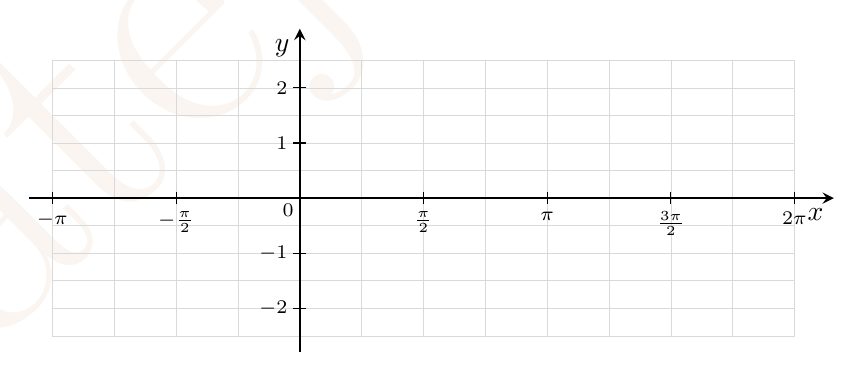
\begin{tikzpicture}[xscale=1,yscale=0.7,>=stealth]
\draw[very thin,gray!30,xstep=0.785398,ystep=0.5] (-3.1416,-2.5) grid (6.2832,2.5);
\draw[->,thick] (-3.4416,0) -- (6.7832,0) node[below left] {$x$};
\draw[->,thick] (0,-2.78571) -- (0,3.07143) node[below left] {$y$};
\draw (-3.1416,0.1143) -- (-3.1416,-0.1143);
\node[below,inner sep=2pt] at (-3.1416,-0.1429) {\scriptsize $-\pi$};
\draw (-1.5708,0.1143) -- (-1.5708,-0.1143);
\node[below,inner sep=2pt] at (-1.5708,-0.1429) {\scriptsize $-\tfrac{\pi}{2}$};
\draw (1.5708,0.1143) -- (1.5708,-0.1143);
\node[below,inner sep=2pt] at (1.5708,-0.1429) {\scriptsize $\tfrac{\pi}{2}$};
\draw (3.1416,0.1143) -- (3.1416,-0.1143);
\node[below,inner sep=2pt] at (3.1416,-0.1429) {\scriptsize $\pi$};
\draw (4.7124,0.1143) -- (4.7124,-0.1143);
\node[below,inner sep=2pt] at (4.7124,-0.1429) {\scriptsize $\tfrac{3\pi}{2}$};
\draw (6.2832,0.1143) -- (6.2832,-0.1143);
\node[below,inner sep=2pt] at (6.2832,-0.1429) {\scriptsize $2\pi$};
\draw (0.0800,-2) -- (-0.0800,-2) node[left,inner sep=2pt] {\scriptsize $-2$};
\draw (0.0800,-1) -- (-0.0800,-1) node[left,inner sep=2pt] {\scriptsize $-1$};
\draw (0.0800,1) -- (-0.0800,1) node[left,inner sep=2pt] {\scriptsize $1$};
\draw (0.0800,2) -- (-0.0800,2) node[left,inner sep=2pt] {\scriptsize $2$};
\node[below left,inner sep=2pt] at (0,0) {\scriptsize $0$};
\end{tikzpicture}
\end{center}
\begin{center}$Z_f=$\,\rule{4cm}{0.1mm}\qquad $\omega=$\,\rule{3cm}{0.1mm}\end{center}

\item $\displaystyle f(x)=-\frac12\cos\Big(2x-\frac{\pi}{2}\Big)$
\begin{center}
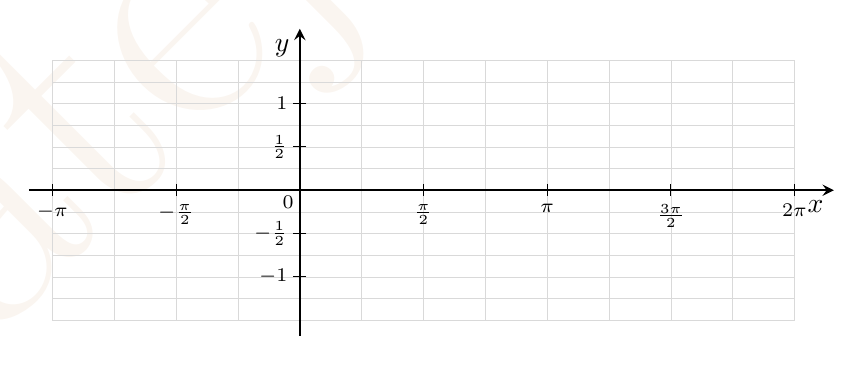
\begin{tikzpicture}[xscale=1,yscale=1.1,>=stealth]
\draw[very thin,gray!30,xstep=0.785398,ystep=0.25] (-3.1416,-1.5) grid (6.2832,1.5);
\draw[->,thick] (-3.4416,0) -- (6.7832,0) node[below left] {$x$};
\draw[->,thick] (0,-1.68182) -- (0,1.86364) node[below left] {$y$};
\draw (-3.1416,0.0727) -- (-3.1416,-0.0727);
\node[below,inner sep=2pt] at (-3.1416,-0.0909) {\scriptsize $-\pi$};
\draw (-1.5708,0.0727) -- (-1.5708,-0.0727);
\node[below,inner sep=2pt] at (-1.5708,-0.0909) {\scriptsize $-\tfrac{\pi}{2}$};
\draw (1.5708,0.0727) -- (1.5708,-0.0727);
\node[below,inner sep=2pt] at (1.5708,-0.0909) {\scriptsize $\tfrac{\pi}{2}$};
\draw (3.1416,0.0727) -- (3.1416,-0.0727);
\node[below,inner sep=2pt] at (3.1416,-0.0909) {\scriptsize $\pi$};
\draw (4.7124,0.0727) -- (4.7124,-0.0727);
\node[below,inner sep=2pt] at (4.7124,-0.0909) {\scriptsize $\tfrac{3\pi}{2}$};
\draw (6.2832,0.0727) -- (6.2832,-0.0727);
\node[below,inner sep=2pt] at (6.2832,-0.0909) {\scriptsize $2\pi$};
\draw (0.0800,-1) -- (-0.0800,-1) node[left,inner sep=2pt] {\scriptsize $-1$};
\draw (0.0800,-0.5) -- (-0.0800,-0.5) node[left,inner sep=2pt] {\scriptsize $-\tfrac12$};
\draw (0.0800,0.5) -- (-0.0800,0.5) node[left,inner sep=2pt] {\scriptsize $\tfrac12$};
\draw (0.0800,1) -- (-0.0800,1) node[left,inner sep=2pt] {\scriptsize $1$};
\node[below left,inner sep=2pt] at (0,0) {\scriptsize $0$};
\end{tikzpicture}
\end{center}
\begin{center}$Z_f=$\,\rule{4cm}{0.1mm}\qquad $\omega=$\,\rule{3cm}{0.1mm}\end{center}

\item $\displaystyle f(x)=3\sin\Big(\frac{x}{2}+\frac{\pi}{3}\Big)+1$
\begin{center}
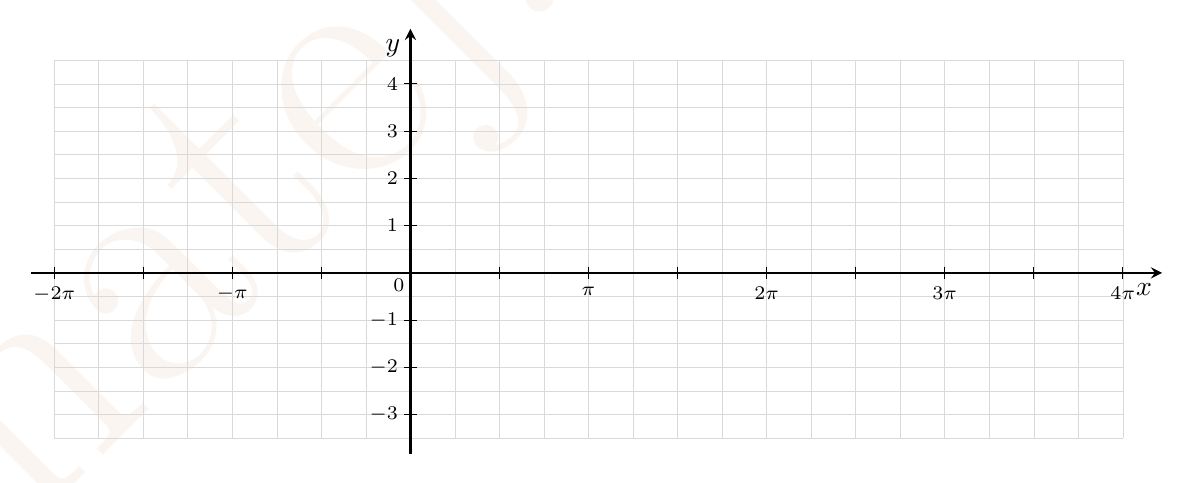
\begin{tikzpicture}[xscale=0.72,yscale=0.6,>=stealth]
\draw[very thin,gray!30,xstep=0.785398,ystep=0.5] (-6.2832,-3.5) grid (12.5664,4.5);
\draw[->,thick] (-6.6999,0) -- (13.2608,0) node[below left] {$x$};
\draw[->,thick] (0,-3.83333) -- (0,5.16667) node[below left] {$y$};
\draw (-6.2832,0.1333) -- (-6.2832,-0.1333);
\node[below,inner sep=2pt] at (-6.2832,-0.1667) {\scriptsize $-2\pi$};
\draw (-4.7124,0.1333) -- (-4.7124,-0.1333);
\draw (-3.1416,0.1333) -- (-3.1416,-0.1333);
\node[below,inner sep=2pt] at (-3.1416,-0.1667) {\scriptsize $-\pi$};
\draw (-1.5708,0.1333) -- (-1.5708,-0.1333);
\draw (1.5708,0.1333) -- (1.5708,-0.1333);
\draw (3.1416,0.1333) -- (3.1416,-0.1333);
\node[below,inner sep=2pt] at (3.1416,-0.1667) {\scriptsize $\pi$};
\draw (4.7124,0.1333) -- (4.7124,-0.1333);
\draw (6.2832,0.1333) -- (6.2832,-0.1333);
\node[below,inner sep=2pt] at (6.2832,-0.1667) {\scriptsize $2\pi$};
\draw (7.8540,0.1333) -- (7.8540,-0.1333);
\draw (9.4248,0.1333) -- (9.4248,-0.1333);
\node[below,inner sep=2pt] at (9.4248,-0.1667) {\scriptsize $3\pi$};
\draw (10.9956,0.1333) -- (10.9956,-0.1333);
\draw (12.5664,0.1333) -- (12.5664,-0.1333);
\node[below,inner sep=2pt] at (12.5664,-0.1667) {\scriptsize $4\pi$};
\draw (0.1111,-3) -- (-0.1111,-3) node[left,inner sep=2pt] {\scriptsize $-3$};
\draw (0.1111,-2) -- (-0.1111,-2) node[left,inner sep=2pt] {\scriptsize $-2$};
\draw (0.1111,-1) -- (-0.1111,-1) node[left,inner sep=2pt] {\scriptsize $-1$};
\draw (0.1111,1) -- (-0.1111,1) node[left,inner sep=2pt] {\scriptsize $1$};
\draw (0.1111,2) -- (-0.1111,2) node[left,inner sep=2pt] {\scriptsize $2$};
\draw (0.1111,3) -- (-0.1111,3) node[left,inner sep=2pt] {\scriptsize $3$};
\draw (0.1111,4) -- (-0.1111,4) node[left,inner sep=2pt] {\scriptsize $4$};
\node[below left,inner sep=2pt] at (0,0) {\scriptsize $0$};
\end{tikzpicture}
\end{center}
\begin{center}$Z_f=$\,\rule{4cm}{0.1mm}\qquad $\omega=$\,\rule{3cm}{0.1mm}\end{center}

\end{enumerate}
\end{naloga}
\newpage

\begin{naloga}[\hfill $\tockeG$] \addtocounter{tocke}{\numexpr\tockeG\relax}
Iz grafa razberi funkcijski predpis funkcije $f$ (oblike $f(x)=A\sin(bx+c)+d$ oziroma $f(x)=A\cos(bx+c)+d$).
\begin{center}
\begin{minipage}[t]{0.48\textwidth}\centering
{\small a)}\\[2pt]
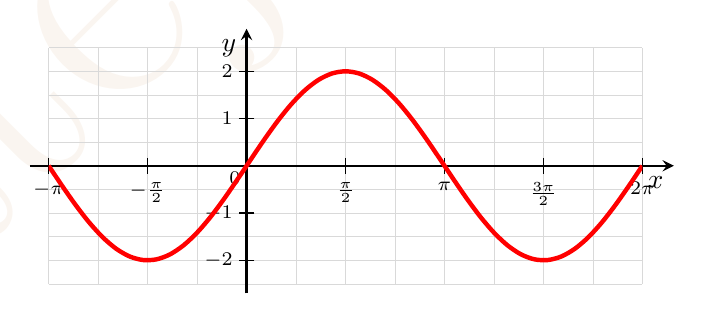
\begin{tikzpicture}[xscale=0.8,yscale=0.6,>=stealth]
\draw[very thin,gray!30,xstep=0.785398,ystep=0.5] (-3.1416,-2.5) grid (6.2832,2.5);
\draw[->,thick] (-3.4416,0) -- (6.7832,0) node[below left] {$x$};
\draw[->,thick] (0,-2.7) -- (0,2.9) node[below left] {$y$};
\draw (-3.1416,0.1667) -- (-3.1416,-0.1667);
\node[below,inner sep=2pt] at (-3.1416,-0.2167) {\scriptsize $-\pi$};
\draw (-1.5708,0.1667) -- (-1.5708,-0.1667);
\node[below,inner sep=2pt] at (-1.5708,-0.2167) {\scriptsize $-\tfrac{\pi}{2}$};
\draw (1.5708,0.1667) -- (1.5708,-0.1667);
\node[below,inner sep=2pt] at (1.5708,-0.2167) {\scriptsize $\tfrac{\pi}{2}$};
\draw (3.1416,0.1667) -- (3.1416,-0.1667);
\node[below,inner sep=2pt] at (3.1416,-0.2167) {\scriptsize $\pi$};
\draw (4.7124,0.1667) -- (4.7124,-0.1667);
\node[below,inner sep=2pt] at (4.7124,-0.2167) {\scriptsize $\tfrac{3\pi}{2}$};
\draw (6.2832,0.1667) -- (6.2832,-0.1667);
\node[below,inner sep=2pt] at (6.2832,-0.2167) {\scriptsize $2\pi$};
\draw (0.1250,-2) -- (-0.1250,-2) node[left,inner sep=2pt] {\scriptsize $-2$};
\draw (0.1250,-1) -- (-0.1250,-1) node[left,inner sep=2pt] {\scriptsize $-1$};
\draw (0.1250,1) -- (-0.1250,1) node[left,inner sep=2pt] {\scriptsize $1$};
\draw (0.1250,2) -- (-0.1250,2) node[left,inner sep=2pt] {\scriptsize $2$};
\node[below left,inner sep=2pt] at (0,0) {\scriptsize $0$};
\begin{scope}
\clip (-3.1416,-2.5) rectangle (6.2832,2.5);
\draw[red,line width=1.6pt,domain=-3.1416:6.2832,samples=45,smooth] plot (\x,{2*sin(deg(\x))});
\end{scope}
\end{tikzpicture}
\\[4pt] $f(x)=$\,\rule{5cm}{0.1mm}
\end{minipage}\hfill
\begin{minipage}[t]{0.48\textwidth}\centering
{\small b)}\\[2pt]
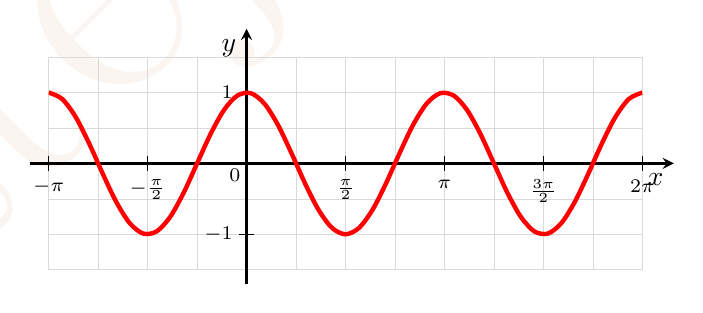
\begin{tikzpicture}[xscale=0.8,yscale=0.9,>=stealth]
\draw[very thin,gray!30,xstep=0.785398,ystep=0.5] (-3.1416,-1.5) grid (6.2832,1.5);
\draw[->,thick] (-3.4416,0) -- (6.7832,0) node[below left] {$x$};
\draw[->,thick] (0,-1.7) -- (0,1.9) node[below left] {$y$};
\draw (-3.1416,0.1111) -- (-3.1416,-0.1111);
\node[below,inner sep=2pt] at (-3.1416,-0.1444) {\scriptsize $-\pi$};
\draw (-1.5708,0.1111) -- (-1.5708,-0.1111);
\node[below,inner sep=2pt] at (-1.5708,-0.1444) {\scriptsize $-\tfrac{\pi}{2}$};
\draw (1.5708,0.1111) -- (1.5708,-0.1111);
\node[below,inner sep=2pt] at (1.5708,-0.1444) {\scriptsize $\tfrac{\pi}{2}$};
\draw (3.1416,0.1111) -- (3.1416,-0.1111);
\node[below,inner sep=2pt] at (3.1416,-0.1444) {\scriptsize $\pi$};
\draw (4.7124,0.1111) -- (4.7124,-0.1111);
\node[below,inner sep=2pt] at (4.7124,-0.1444) {\scriptsize $\tfrac{3\pi}{2}$};
\draw (6.2832,0.1111) -- (6.2832,-0.1111);
\node[below,inner sep=2pt] at (6.2832,-0.1444) {\scriptsize $2\pi$};
\draw (0.1250,-1) -- (-0.1250,-1) node[left,inner sep=2pt] {\scriptsize $-1$};
\draw (0.1250,1) -- (-0.1250,1) node[left,inner sep=2pt] {\scriptsize $1$};
\node[below left,inner sep=2pt] at (0,0) {\scriptsize $0$};
\begin{scope}
\clip (-3.1416,-1.5) rectangle (6.2832,1.5);
\draw[red,line width=1.6pt,domain=-3.1416:6.2832,samples=45,smooth] plot (\x,{cos(deg(2*\x))});
\end{scope}
\end{tikzpicture}
\\[4pt] $f(x)=$\,\rule{5cm}{0.1mm}
\end{minipage}\\[0.6cm]
\begin{minipage}[t]{0.48\textwidth}\centering
{\small c)}\\[2pt]
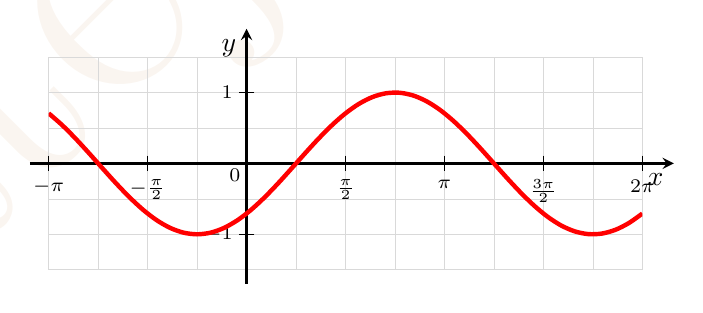
\begin{tikzpicture}[xscale=0.8,yscale=0.9,>=stealth]
\draw[very thin,gray!30,xstep=0.785398,ystep=0.5] (-3.1416,-1.5) grid (6.2832,1.5);
\draw[->,thick] (-3.4416,0) -- (6.7832,0) node[below left] {$x$};
\draw[->,thick] (0,-1.7) -- (0,1.9) node[below left] {$y$};
\draw (-3.1416,0.1111) -- (-3.1416,-0.1111);
\node[below,inner sep=2pt] at (-3.1416,-0.1444) {\scriptsize $-\pi$};
\draw (-1.5708,0.1111) -- (-1.5708,-0.1111);
\node[below,inner sep=2pt] at (-1.5708,-0.1444) {\scriptsize $-\tfrac{\pi}{2}$};
\draw (1.5708,0.1111) -- (1.5708,-0.1111);
\node[below,inner sep=2pt] at (1.5708,-0.1444) {\scriptsize $\tfrac{\pi}{2}$};
\draw (3.1416,0.1111) -- (3.1416,-0.1111);
\node[below,inner sep=2pt] at (3.1416,-0.1444) {\scriptsize $\pi$};
\draw (4.7124,0.1111) -- (4.7124,-0.1111);
\node[below,inner sep=2pt] at (4.7124,-0.1444) {\scriptsize $\tfrac{3\pi}{2}$};
\draw (6.2832,0.1111) -- (6.2832,-0.1111);
\node[below,inner sep=2pt] at (6.2832,-0.1444) {\scriptsize $2\pi$};
\draw (0.1250,-1) -- (-0.1250,-1) node[left,inner sep=2pt] {\scriptsize $-1$};
\draw (0.1250,1) -- (-0.1250,1) node[left,inner sep=2pt] {\scriptsize $1$};
\node[below left,inner sep=2pt] at (0,0) {\scriptsize $0$};
\begin{scope}
\clip (-3.1416,-1.5) rectangle (6.2832,1.5);
\draw[red,line width=1.6pt,domain=-3.1416:6.2832,samples=45,smooth] plot (\x,{sin(deg(\x-pi/4))});
\end{scope}
\end{tikzpicture}
\\[4pt] $f(x)=$\,\rule{5cm}{0.1mm}
\end{minipage}\hfill
\begin{minipage}[t]{0.48\textwidth}\centering
{\small d)}\\[2pt]
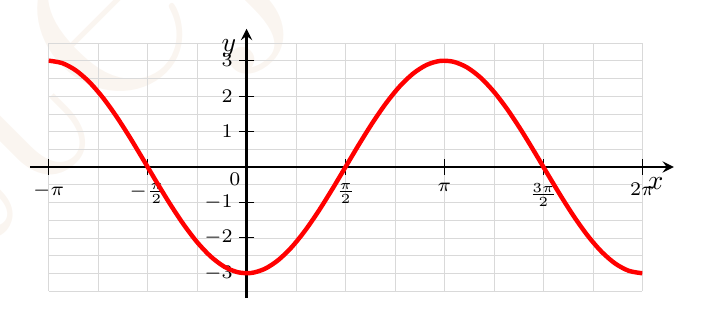
\begin{tikzpicture}[xscale=0.8,yscale=0.45,>=stealth]
\draw[very thin,gray!30,xstep=0.785398,ystep=0.5] (-3.1416,-3.5) grid (6.2832,3.5);
\draw[->,thick] (-3.4416,0) -- (6.7832,0) node[below left] {$x$};
\draw[->,thick] (0,-3.7) -- (0,3.9) node[below left] {$y$};
\draw (-3.1416,0.2222) -- (-3.1416,-0.2222);
\node[below,inner sep=2pt] at (-3.1416,-0.2889) {\scriptsize $-\pi$};
\draw (-1.5708,0.2222) -- (-1.5708,-0.2222);
\node[below,inner sep=2pt] at (-1.5708,-0.2889) {\scriptsize $-\tfrac{\pi}{2}$};
\draw (1.5708,0.2222) -- (1.5708,-0.2222);
\node[below,inner sep=2pt] at (1.5708,-0.2889) {\scriptsize $\tfrac{\pi}{2}$};
\draw (3.1416,0.2222) -- (3.1416,-0.2222);
\node[below,inner sep=2pt] at (3.1416,-0.2889) {\scriptsize $\pi$};
\draw (4.7124,0.2222) -- (4.7124,-0.2222);
\node[below,inner sep=2pt] at (4.7124,-0.2889) {\scriptsize $\tfrac{3\pi}{2}$};
\draw (6.2832,0.2222) -- (6.2832,-0.2222);
\node[below,inner sep=2pt] at (6.2832,-0.2889) {\scriptsize $2\pi$};
\draw (0.1250,-3) -- (-0.1250,-3) node[left,inner sep=2pt] {\scriptsize $-3$};
\draw (0.1250,-2) -- (-0.1250,-2) node[left,inner sep=2pt] {\scriptsize $-2$};
\draw (0.1250,-1) -- (-0.1250,-1) node[left,inner sep=2pt] {\scriptsize $-1$};
\draw (0.1250,1) -- (-0.1250,1) node[left,inner sep=2pt] {\scriptsize $1$};
\draw (0.1250,2) -- (-0.1250,2) node[left,inner sep=2pt] {\scriptsize $2$};
\draw (0.1250,3) -- (-0.1250,3) node[left,inner sep=2pt] {\scriptsize $3$};
\node[below left,inner sep=2pt] at (0,0) {\scriptsize $0$};
\begin{scope}
\clip (-3.1416,-3.5) rectangle (6.2832,3.5);
\draw[red,line width=1.6pt,domain=-3.1416:6.2832,samples=45,smooth] plot (\x,{-3*cos(deg(\x))});
\end{scope}
\end{tikzpicture}
\\[4pt] $f(x)=$\,\rule{5cm}{0.1mm}
\end{minipage}\\[0.6cm]
\begin{minipage}[t]{0.48\textwidth}\centering
{\small e)}\\[2pt]
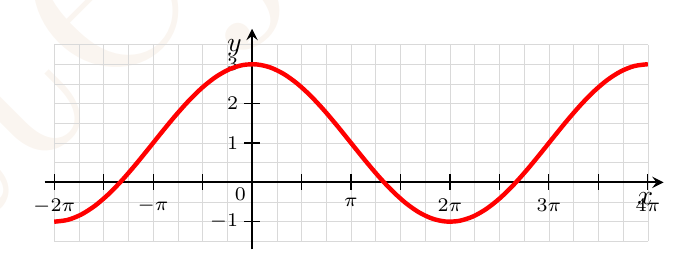
\begin{tikzpicture}[xscale=0.4,yscale=0.5,>=stealth]
\draw[very thin,gray!30,xstep=0.785398,ystep=0.5] (-6.2832,-1.5) grid (12.5664,3.5);
\draw[->,thick] (-6.5832,0) -- (13.0664,0) node[below left] {$x$};
\draw[->,thick] (0,-1.7) -- (0,3.9) node[below left] {$y$};
\draw (-6.2832,0.2000) -- (-6.2832,-0.2000);
\node[below,inner sep=2pt] at (-6.2832,-0.2600) {\scriptsize $-2\pi$};
\draw (-4.7124,0.2000) -- (-4.7124,-0.2000);
\draw (-3.1416,0.2000) -- (-3.1416,-0.2000);
\node[below,inner sep=2pt] at (-3.1416,-0.2600) {\scriptsize $-\pi$};
\draw (-1.5708,0.2000) -- (-1.5708,-0.2000);
\draw (1.5708,0.2000) -- (1.5708,-0.2000);
\draw (3.1416,0.2000) -- (3.1416,-0.2000);
\node[below,inner sep=2pt] at (3.1416,-0.2600) {\scriptsize $\pi$};
\draw (4.7124,0.2000) -- (4.7124,-0.2000);
\draw (6.2832,0.2000) -- (6.2832,-0.2000);
\node[below,inner sep=2pt] at (6.2832,-0.2600) {\scriptsize $2\pi$};
\draw (7.8540,0.2000) -- (7.8540,-0.2000);
\draw (9.4248,0.2000) -- (9.4248,-0.2000);
\node[below,inner sep=2pt] at (9.4248,-0.2600) {\scriptsize $3\pi$};
\draw (10.9956,0.2000) -- (10.9956,-0.2000);
\draw (12.5664,0.2000) -- (12.5664,-0.2000);
\node[below,inner sep=2pt] at (12.5664,-0.2600) {\scriptsize $4\pi$};
\draw (0.2500,-1) -- (-0.2500,-1) node[left,inner sep=2pt] {\scriptsize $-1$};
\draw (0.2500,1) -- (-0.2500,1) node[left,inner sep=2pt] {\scriptsize $1$};
\draw (0.2500,2) -- (-0.2500,2) node[left,inner sep=2pt] {\scriptsize $2$};
\draw (0.2500,3) -- (-0.2500,3) node[left,inner sep=2pt] {\scriptsize $3$};
\node[below left,inner sep=2pt] at (0,0) {\scriptsize $0$};
\begin{scope}
\clip (-6.2832,-1.5) rectangle (12.5664,3.5);
\draw[red,line width=1.6pt,domain=-6.2832:12.5664,samples=45,smooth] plot (\x,{2*cos(deg(\x/2))+1});
\end{scope}
\end{tikzpicture}
\\[4pt] $f(x)=$\,\rule{5cm}{0.1mm}
\end{minipage}\hfill
\begin{minipage}[t]{0.48\textwidth}\centering
{\small f)}\\[2pt]
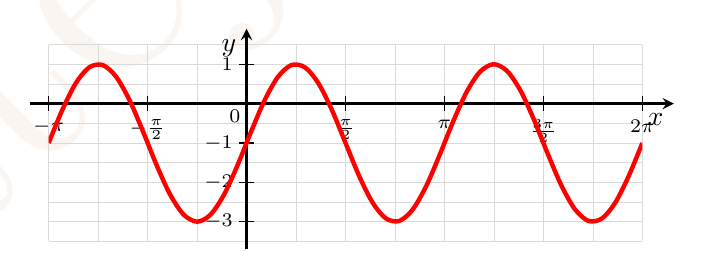
\begin{tikzpicture}[xscale=0.8,yscale=0.5,>=stealth]
\draw[very thin,gray!30,xstep=0.785398,ystep=0.5] (-3.1416,-3.5) grid (6.2832,1.5);
\draw[->,thick] (-3.4416,0) -- (6.7832,0) node[below left] {$x$};
\draw[->,thick] (0,-3.7) -- (0,1.9) node[below left] {$y$};
\draw (-3.1416,0.2000) -- (-3.1416,-0.2000);
\node[below,inner sep=2pt] at (-3.1416,-0.2600) {\scriptsize $-\pi$};
\draw (-1.5708,0.2000) -- (-1.5708,-0.2000);
\node[below,inner sep=2pt] at (-1.5708,-0.2600) {\scriptsize $-\tfrac{\pi}{2}$};
\draw (1.5708,0.2000) -- (1.5708,-0.2000);
\node[below,inner sep=2pt] at (1.5708,-0.2600) {\scriptsize $\tfrac{\pi}{2}$};
\draw (3.1416,0.2000) -- (3.1416,-0.2000);
\node[below,inner sep=2pt] at (3.1416,-0.2600) {\scriptsize $\pi$};
\draw (4.7124,0.2000) -- (4.7124,-0.2000);
\node[below,inner sep=2pt] at (4.7124,-0.2600) {\scriptsize $\tfrac{3\pi}{2}$};
\draw (6.2832,0.2000) -- (6.2832,-0.2000);
\node[below,inner sep=2pt] at (6.2832,-0.2600) {\scriptsize $2\pi$};
\draw (0.1250,-3) -- (-0.1250,-3) node[left,inner sep=2pt] {\scriptsize $-3$};
\draw (0.1250,-2) -- (-0.1250,-2) node[left,inner sep=2pt] {\scriptsize $-2$};
\draw (0.1250,-1) -- (-0.1250,-1) node[left,inner sep=2pt] {\scriptsize $-1$};
\draw (0.1250,1) -- (-0.1250,1) node[left,inner sep=2pt] {\scriptsize $1$};
\node[below left,inner sep=2pt] at (0,0) {\scriptsize $0$};
\begin{scope}
\clip (-3.1416,-3.5) rectangle (6.2832,1.5);
\draw[red,line width=1.6pt,domain=-3.1416:6.2832,samples=45,smooth] plot (\x,{2*sin(deg(2*\x))-1});
\end{scope}
\end{tikzpicture}
\\[4pt] $f(x)=$\,\rule{5cm}{0.1mm}
\end{minipage}\\[0.6cm]
\end{center}
\end{naloga}
\newpage

\begin{naloga}[\hfill $\tockeC$] \addtocounter{tocke}{\numexpr\tockeC\relax}
Dolo\v{c}i osnovno periodo in zalogo vrednosti funkcije $\displaystyle y=5-10\cos^2x$ ter abscise maksimumov.
\vspace{3.5cm}
\end{naloga}

\begin{naloga}[\hfill $\tockeD$] \addtocounter{tocke}{\numexpr\tockeD\relax}
Dolo\v{c}i osnovno periodo in zalogo vrednosti funkcije $\displaystyle y=2-4\sin^2x$ ter abscise minimumov.
\vspace{3.5cm}
\end{naloga}

\begin{naloga}[\hfill $\tockeE$] \addtocounter{tocke}{\numexpr\tockeE\relax}
Funkcijo $\displaystyle y=2\sin2x-2\sqrt3\cos2x$ zapi\v{s}i v obliki $y=A\sin(\omega x+\varphi)$. Dolo\v{c}i osnovno periodo, zalogo vrednosti in za\v{c}etno vrednost.
\vspace{4cm}
\end{naloga}

\begin{naloga}[\hfill $\tockeF$] \addtocounter{tocke}{\numexpr\tockeF\relax}
Funkcijo $\displaystyle y=\sqrt3\cos2x-\sin2x$ zapi\v{s}i v obliki $y=A\cos(\omega x+\varphi)$. Dolo\v{c}i osnovno periodo, zalogo vrednosti in za\v{c}etno vrednost.
\vspace{4cm}
\end{naloga}

\end{document}

\newpage
\textsc{\Large Re\v{s}itve}
\vspace{0.5cm}

\begin{resitev}[-- Zahtevnej\v{s}e naloge]
\begin{enumerate}[a)]
\item $\displaystyle \sin3x-\sin2x=2\cos\tfrac{5x}{2}\sin\tfrac{x}{2}\ \Rightarrow\ \frac{2\cos\frac{5x}{2}\sin\frac{x}{2}\cos\frac{x}{2}}{\cos\frac{5x}{2}}=2\sin\tfrac{x}{2}\cos\tfrac{x}{2}=\sin x$
\item $\displaystyle 2\sin33\degree\sin27\degree=\cos6\degree-\cos60\degree=\cos6\degree-\tfrac12$;\quad
$\displaystyle 2\cos3\degree\big(\cos6\degree-\tfrac12\big)=\cos9\degree+\cos3\degree-\cos3\degree=\cos9\degree$
\item $\displaystyle 2\sin20\degree\sin40\degree=\cos20\degree-\tfrac12$;\quad
$\displaystyle \big(\cos20\degree-\tfrac12\big)\sin80\degree=\tfrac12(\sin100\degree+\sin60\degree)-\tfrac12\sin80\degree=\tfrac12\sin60\degree=\tfrac{\sqrt3}{4}$, torej produkt $=\tfrac{\sqrt3}{8}$
\item $\displaystyle 8\sin20\degree\cos20\degree\cos40\degree\cos80\degree=4\sin40\degree\cos40\degree\cos80\degree=2\sin80\degree\cos80\degree=\sin160\degree=\sin20\degree\ \Rightarrow\ \frac18$
\item $\displaystyle \frac{2\sin3x\cos2x+\sin3x}{2\cos3x\cos2x+\cos3x}=\frac{\sin3x\,(2\cos2x+1)}{\cos3x\,(2\cos2x+1)}=\tan3x$
\item $\displaystyle \frac{2\sin2x\sin x}{2\cos2x\sin x}=\tan2x$
\item $\displaystyle \cos^273\degree+\cos^247\degree=1+\cos120\degree\cos26\degree=1-\tfrac12\cos26\degree$;\quad $\cos73\degree\cos47\degree=-\tfrac14+\tfrac12\cos26\degree$;\quad vsota $=\dfrac34$
\item $\displaystyle \tan(\alpha+\beta)=1\Rightarrow \tan\alpha+\tan\beta=1-\tan\alpha\tan\beta$;\quad $(1+\tan\alpha)(1+\tan\beta)=1+(1-\tan\alpha\tan\beta)+\tan\alpha\tan\beta=2$
\end{enumerate}
\end{resitev}

\begin{resitev}[-- Grafi kotnih funkcij]
\begin{enumerate}[a)]
\item Graf $y=\sin x$ premaknemo za $\frac{\pi}{4}$ v levo. \quad $Z_f=[-1,1]$, \ $\omega=2\pi$
\begin{center}
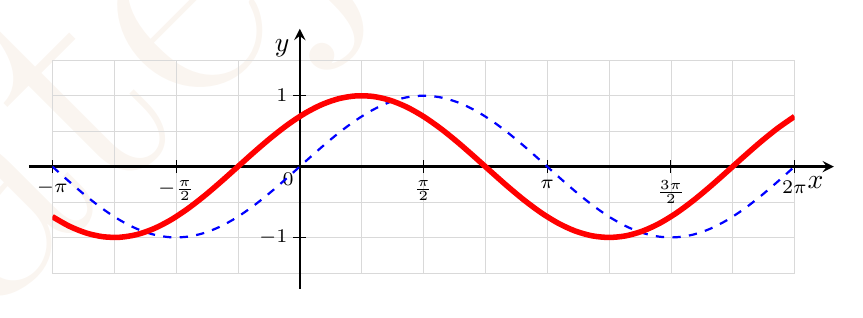
\begin{tikzpicture}[xscale=1,yscale=0.9,>=stealth]
\draw[very thin,gray!30,xstep=0.785398,ystep=0.5] (-3.1416,-1.5) grid (6.2832,1.5);
\draw[->,thick] (-3.4416,0) -- (6.7832,0) node[below left] {$x$};
\draw[->,thick] (0,-1.72222) -- (0,1.94444) node[below left] {$y$};
\draw (-3.1416,0.0889) -- (-3.1416,-0.0889);
\node[below,inner sep=2pt] at (-3.1416,-0.1111) {\scriptsize $-\pi$};
\draw (-1.5708,0.0889) -- (-1.5708,-0.0889);
\node[below,inner sep=2pt] at (-1.5708,-0.1111) {\scriptsize $-\tfrac{\pi}{2}$};
\draw (1.5708,0.0889) -- (1.5708,-0.0889);
\node[below,inner sep=2pt] at (1.5708,-0.1111) {\scriptsize $\tfrac{\pi}{2}$};
\draw (3.1416,0.0889) -- (3.1416,-0.0889);
\node[below,inner sep=2pt] at (3.1416,-0.1111) {\scriptsize $\pi$};
\draw (4.7124,0.0889) -- (4.7124,-0.0889);
\node[below,inner sep=2pt] at (4.7124,-0.1111) {\scriptsize $\tfrac{3\pi}{2}$};
\draw (6.2832,0.0889) -- (6.2832,-0.0889);
\node[below,inner sep=2pt] at (6.2832,-0.1111) {\scriptsize $2\pi$};
\draw (0.0800,-1) -- (-0.0800,-1) node[left,inner sep=2pt] {\scriptsize $-1$};
\draw (0.0800,1) -- (-0.0800,1) node[left,inner sep=2pt] {\scriptsize $1$};
\node[below left,inner sep=2pt] at (0,0) {\scriptsize $0$};
\begin{scope}
\clip (-3.1416,-1.5) rectangle (6.2832,1.5);
\draw[blue,dashed,thick,domain=-3.1416:6.2832,samples=45,smooth] plot (\x,{sin(deg(\x))});
\draw[red,line width=2pt,domain=-3.1416:6.2832,samples=45,smooth] plot (\x,{sin(deg(\x+pi/4))});
\end{scope}
\end{tikzpicture}
\end{center}
\begin{center}\small \tikz[baseline=-0.6ex]\draw[blue,dashed,thick] (0,0)--(0.8,0);\ $y=\sin x$ \quad \tikz[baseline=-0.6ex]\draw[red,line width=2pt] (0,0)--(0.8,0);\ $f(x)=\sin\big(x+\tfrac{\pi}{4}\big)$\end{center}

\item Graf $y=\cos x$ premaknemo za $\frac{\pi}{3}$ v desno. \quad $Z_f=[-1,1]$, \ $\omega=2\pi$
\begin{center}
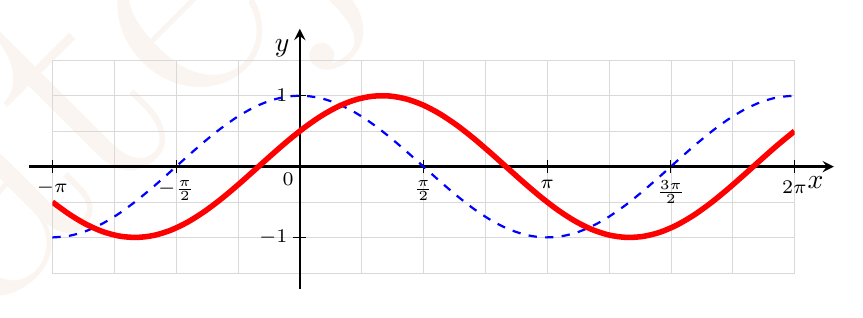
\begin{tikzpicture}[xscale=1,yscale=0.9,>=stealth]
\draw[very thin,gray!30,xstep=0.785398,ystep=0.5] (-3.1416,-1.5) grid (6.2832,1.5);
\draw[->,thick] (-3.4416,0) -- (6.7832,0) node[below left] {$x$};
\draw[->,thick] (0,-1.72222) -- (0,1.94444) node[below left] {$y$};
\draw (-3.1416,0.0889) -- (-3.1416,-0.0889);
\node[below,inner sep=2pt] at (-3.1416,-0.1111) {\scriptsize $-\pi$};
\draw (-1.5708,0.0889) -- (-1.5708,-0.0889);
\node[below,inner sep=2pt] at (-1.5708,-0.1111) {\scriptsize $-\tfrac{\pi}{2}$};
\draw (1.5708,0.0889) -- (1.5708,-0.0889);
\node[below,inner sep=2pt] at (1.5708,-0.1111) {\scriptsize $\tfrac{\pi}{2}$};
\draw (3.1416,0.0889) -- (3.1416,-0.0889);
\node[below,inner sep=2pt] at (3.1416,-0.1111) {\scriptsize $\pi$};
\draw (4.7124,0.0889) -- (4.7124,-0.0889);
\node[below,inner sep=2pt] at (4.7124,-0.1111) {\scriptsize $\tfrac{3\pi}{2}$};
\draw (6.2832,0.0889) -- (6.2832,-0.0889);
\node[below,inner sep=2pt] at (6.2832,-0.1111) {\scriptsize $2\pi$};
\draw (0.0800,-1) -- (-0.0800,-1) node[left,inner sep=2pt] {\scriptsize $-1$};
\draw (0.0800,1) -- (-0.0800,1) node[left,inner sep=2pt] {\scriptsize $1$};
\node[below left,inner sep=2pt] at (0,0) {\scriptsize $0$};
\begin{scope}
\clip (-3.1416,-1.5) rectangle (6.2832,1.5);
\draw[blue,dashed,thick,domain=-3.1416:6.2832,samples=45,smooth] plot (\x,{cos(deg(\x))});
\draw[red,line width=2pt,domain=-3.1416:6.2832,samples=45,smooth] plot (\x,{cos(deg(\x-pi/3))});
\end{scope}
\end{tikzpicture}
\end{center}
\begin{center}\small \tikz[baseline=-0.6ex]\draw[blue,dashed,thick] (0,0)--(0.8,0);\ $y=\cos x$ \quad \tikz[baseline=-0.6ex]\draw[red,line width=2pt] (0,0)--(0.8,0);\ $f(x)=\cos\big(x-\tfrac{\pi}{3}\big)$\end{center}

\newpage
\item $Z_f=[-2,2]$, \ $\omega=2\pi$
\[y=\sin x\ \xrightarrow{\ \frac{\pi}{6}\text{ levo}\ }\ y=\sin\big(x+\tfrac{\pi}{6}\big)\ \xrightarrow{\ \text{razteg v smeri }y\ (\cdot 2)\ }\ f(x)=2\sin\big(x+\tfrac{\pi}{6}\big)\]
\begin{center}
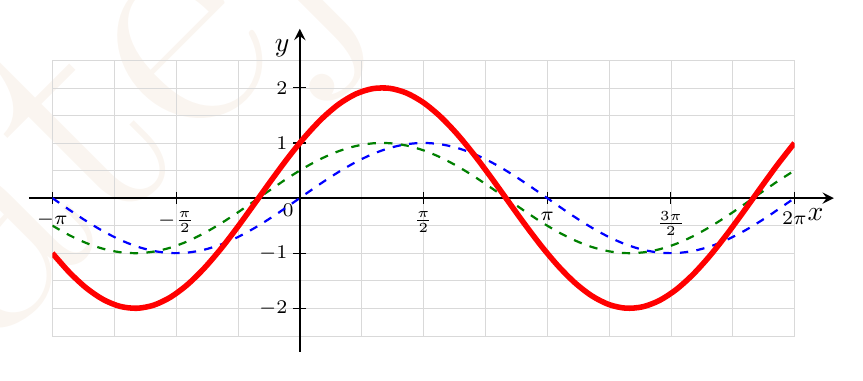
\begin{tikzpicture}[xscale=1,yscale=0.7,>=stealth]
\draw[very thin,gray!30,xstep=0.785398,ystep=0.5] (-3.1416,-2.5) grid (6.2832,2.5);
\draw[->,thick] (-3.4416,0) -- (6.7832,0) node[below left] {$x$};
\draw[->,thick] (0,-2.78571) -- (0,3.07143) node[below left] {$y$};
\draw (-3.1416,0.1143) -- (-3.1416,-0.1143);
\node[below,inner sep=2pt] at (-3.1416,-0.1429) {\scriptsize $-\pi$};
\draw (-1.5708,0.1143) -- (-1.5708,-0.1143);
\node[below,inner sep=2pt] at (-1.5708,-0.1429) {\scriptsize $-\tfrac{\pi}{2}$};
\draw (1.5708,0.1143) -- (1.5708,-0.1143);
\node[below,inner sep=2pt] at (1.5708,-0.1429) {\scriptsize $\tfrac{\pi}{2}$};
\draw (3.1416,0.1143) -- (3.1416,-0.1143);
\node[below,inner sep=2pt] at (3.1416,-0.1429) {\scriptsize $\pi$};
\draw (4.7124,0.1143) -- (4.7124,-0.1143);
\node[below,inner sep=2pt] at (4.7124,-0.1429) {\scriptsize $\tfrac{3\pi}{2}$};
\draw (6.2832,0.1143) -- (6.2832,-0.1143);
\node[below,inner sep=2pt] at (6.2832,-0.1429) {\scriptsize $2\pi$};
\draw (0.0800,-2) -- (-0.0800,-2) node[left,inner sep=2pt] {\scriptsize $-2$};
\draw (0.0800,-1) -- (-0.0800,-1) node[left,inner sep=2pt] {\scriptsize $-1$};
\draw (0.0800,1) -- (-0.0800,1) node[left,inner sep=2pt] {\scriptsize $1$};
\draw (0.0800,2) -- (-0.0800,2) node[left,inner sep=2pt] {\scriptsize $2$};
\node[below left,inner sep=2pt] at (0,0) {\scriptsize $0$};
\begin{scope}
\clip (-3.1416,-2.5) rectangle (6.2832,2.5);
\draw[blue,dashed,thick,domain=-3.1416:6.2832,samples=45,smooth] plot (\x,{sin(deg(\x))});
\draw[green!50!black,dashed,thick,domain=-3.1416:6.2832,samples=45,smooth] plot (\x,{sin(deg(\x+pi/6))});
\draw[red,line width=2pt,domain=-3.1416:6.2832,samples=45,smooth] plot (\x,{2*sin(deg(\x+pi/6))});
\end{scope}
\end{tikzpicture}
\end{center}
\begin{center}\small \tikz[baseline=-0.6ex]\draw[blue,dashed,thick] (0,0)--(0.8,0);\ $y=\sin x$ \quad \tikz[baseline=-0.6ex]\draw[green!50!black,dashed,thick] (0,0)--(0.8,0);\ $y=\sin\big(x+\tfrac{\pi}{6}\big)$ \quad \tikz[baseline=-0.6ex]\draw[red,line width=2pt] (0,0)--(0.8,0);\ $f(x)=2\sin\big(x+\tfrac{\pi}{6}\big)$\end{center}

\item $\cos\big(2x-\frac{\pi}{2}\big)=\cos 2\big(x-\frac{\pi}{4}\big)$:
\[y=\cos x\xrightarrow{\text{skr\v{c}ek v smeri }x\ (\cdot\frac12)}\cos2x\xrightarrow{\frac{\pi}{4}\text{ desno}}\cos\big(2x-\tfrac{\pi}{2}\big)\xrightarrow{\ \cdot\frac12\ }\tfrac12\cos\big(2x-\tfrac{\pi}{2}\big)\xrightarrow{\text{zrcaljenje \v{c}ez os }x} f(x)\]
(Opomba: $\cos\big(2x-\frac{\pi}{2}\big)=\sin2x$, torej $f(x)=-\frac12\sin2x$.) \quad $Z_f=\big[-\frac12,\frac12\big]$, \ $\omega=\pi$
\begin{center}
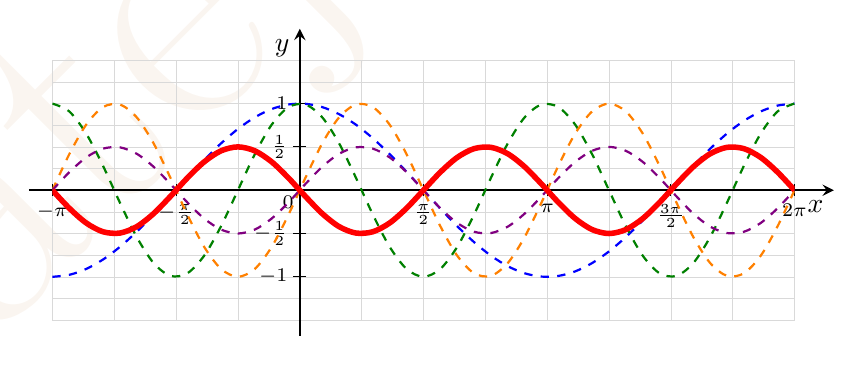
\begin{tikzpicture}[xscale=1,yscale=1.1,>=stealth]
\draw[very thin,gray!30,xstep=0.785398,ystep=0.25] (-3.1416,-1.5) grid (6.2832,1.5);
\draw[->,thick] (-3.4416,0) -- (6.7832,0) node[below left] {$x$};
\draw[->,thick] (0,-1.68182) -- (0,1.86364) node[below left] {$y$};
\draw (-3.1416,0.0727) -- (-3.1416,-0.0727);
\node[below,inner sep=2pt] at (-3.1416,-0.0909) {\scriptsize $-\pi$};
\draw (-1.5708,0.0727) -- (-1.5708,-0.0727);
\node[below,inner sep=2pt] at (-1.5708,-0.0909) {\scriptsize $-\tfrac{\pi}{2}$};
\draw (1.5708,0.0727) -- (1.5708,-0.0727);
\node[below,inner sep=2pt] at (1.5708,-0.0909) {\scriptsize $\tfrac{\pi}{2}$};
\draw (3.1416,0.0727) -- (3.1416,-0.0727);
\node[below,inner sep=2pt] at (3.1416,-0.0909) {\scriptsize $\pi$};
\draw (4.7124,0.0727) -- (4.7124,-0.0727);
\node[below,inner sep=2pt] at (4.7124,-0.0909) {\scriptsize $\tfrac{3\pi}{2}$};
\draw (6.2832,0.0727) -- (6.2832,-0.0727);
\node[below,inner sep=2pt] at (6.2832,-0.0909) {\scriptsize $2\pi$};
\draw (0.0800,-1) -- (-0.0800,-1) node[left,inner sep=2pt] {\scriptsize $-1$};
\draw (0.0800,-0.5) -- (-0.0800,-0.5) node[left,inner sep=2pt] {\scriptsize $-\tfrac12$};
\draw (0.0800,0.5) -- (-0.0800,0.5) node[left,inner sep=2pt] {\scriptsize $\tfrac12$};
\draw (0.0800,1) -- (-0.0800,1) node[left,inner sep=2pt] {\scriptsize $1$};
\node[below left,inner sep=2pt] at (0,0) {\scriptsize $0$};
\begin{scope}
\clip (-3.1416,-1.5) rectangle (6.2832,1.5);
\draw[blue,dashed,thick,domain=-3.1416:6.2832,samples=45,smooth] plot (\x,{cos(deg(\x))});
\draw[green!50!black,dashed,thick,domain=-3.1416:6.2832,samples=45,smooth] plot (\x,{cos(deg(2*\x))});
\draw[orange,dashed,thick,domain=-3.1416:6.2832,samples=45,smooth] plot (\x,{cos(deg(2*\x-pi/2))});
\draw[violet,dashed,thick,domain=-3.1416:6.2832,samples=45,smooth] plot (\x,{0.5*cos(deg(2*\x-pi/2))});
\draw[red,line width=2pt,domain=-3.1416:6.2832,samples=45,smooth] plot (\x,{-0.5*cos(deg(2*\x-pi/2))});
\end{scope}
\end{tikzpicture}
\end{center}
\begin{center}\small \tikz[baseline=-0.6ex]\draw[blue,dashed,thick] (0,0)--(0.8,0);\ $y=\cos x$ \quad \tikz[baseline=-0.6ex]\draw[green!50!black,dashed,thick] (0,0)--(0.8,0);\ $y=\cos 2x$ \quad \tikz[baseline=-0.6ex]\draw[orange,dashed,thick] (0,0)--(0.8,0);\ $y=\cos\big(2x-\tfrac{\pi}{2}\big)$ \\[2pt] \tikz[baseline=-0.6ex]\draw[violet,dashed,thick] (0,0)--(0.8,0);\ $y=\tfrac12\cos\big(2x-\tfrac{\pi}{2}\big)$ \quad \tikz[baseline=-0.6ex]\draw[red,line width=2pt] (0,0)--(0.8,0);\ $f(x)=-\tfrac12\cos\big(2x-\tfrac{\pi}{2}\big)$\end{center}

\newpage
\item $\frac{x}{2}+\frac{\pi}{3}=\frac12\big(x+\frac{2\pi}{3}\big)$:
\[y=\sin x\xrightarrow{\text{razteg v smeri }x\ (\cdot2)}\sin\tfrac{x}{2}\xrightarrow{\frac{2\pi}{3}\text{ levo}}\sin\big(\tfrac{x}{2}+\tfrac{\pi}{3}\big)\xrightarrow{\text{razteg v smeri }y\ (\cdot3)}3\sin\big(\tfrac{x}{2}+\tfrac{\pi}{3}\big)\xrightarrow{\text{za }1\text{ gor}} f(x)\]
$Z_f=[-2,4]$, \ $\omega=4\pi$
\begin{center}
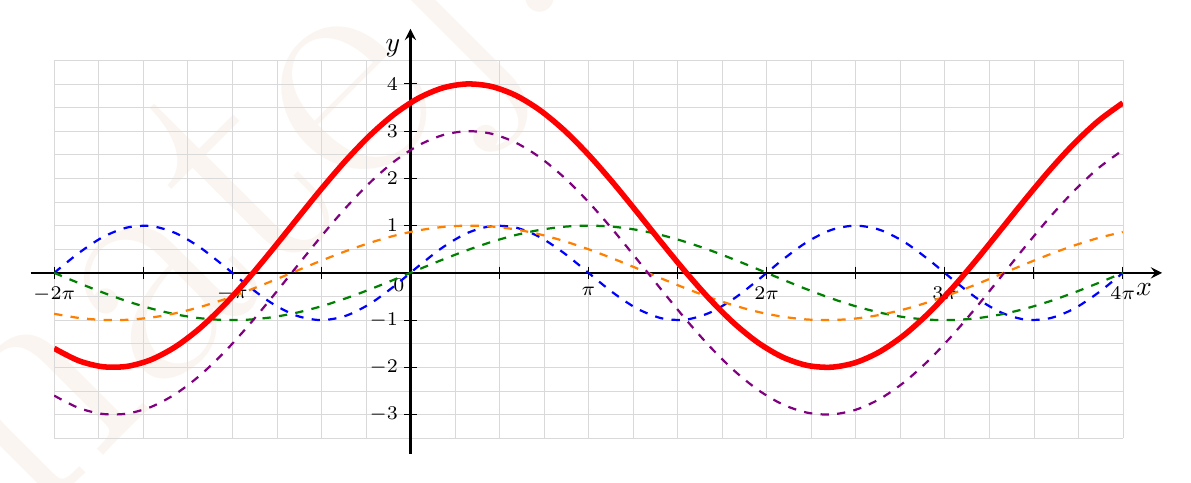
\begin{tikzpicture}[xscale=0.72,yscale=0.6,>=stealth]
\draw[very thin,gray!30,xstep=0.785398,ystep=0.5] (-6.2832,-3.5) grid (12.5664,4.5);
\draw[->,thick] (-6.6999,0) -- (13.2608,0) node[below left] {$x$};
\draw[->,thick] (0,-3.83333) -- (0,5.16667) node[below left] {$y$};
\draw (-6.2832,0.1333) -- (-6.2832,-0.1333);
\node[below,inner sep=2pt] at (-6.2832,-0.1667) {\scriptsize $-2\pi$};
\draw (-4.7124,0.1333) -- (-4.7124,-0.1333);
\draw (-3.1416,0.1333) -- (-3.1416,-0.1333);
\node[below,inner sep=2pt] at (-3.1416,-0.1667) {\scriptsize $-\pi$};
\draw (-1.5708,0.1333) -- (-1.5708,-0.1333);
\draw (1.5708,0.1333) -- (1.5708,-0.1333);
\draw (3.1416,0.1333) -- (3.1416,-0.1333);
\node[below,inner sep=2pt] at (3.1416,-0.1667) {\scriptsize $\pi$};
\draw (4.7124,0.1333) -- (4.7124,-0.1333);
\draw (6.2832,0.1333) -- (6.2832,-0.1333);
\node[below,inner sep=2pt] at (6.2832,-0.1667) {\scriptsize $2\pi$};
\draw (7.8540,0.1333) -- (7.8540,-0.1333);
\draw (9.4248,0.1333) -- (9.4248,-0.1333);
\node[below,inner sep=2pt] at (9.4248,-0.1667) {\scriptsize $3\pi$};
\draw (10.9956,0.1333) -- (10.9956,-0.1333);
\draw (12.5664,0.1333) -- (12.5664,-0.1333);
\node[below,inner sep=2pt] at (12.5664,-0.1667) {\scriptsize $4\pi$};
\draw (0.1111,-3) -- (-0.1111,-3) node[left,inner sep=2pt] {\scriptsize $-3$};
\draw (0.1111,-2) -- (-0.1111,-2) node[left,inner sep=2pt] {\scriptsize $-2$};
\draw (0.1111,-1) -- (-0.1111,-1) node[left,inner sep=2pt] {\scriptsize $-1$};
\draw (0.1111,1) -- (-0.1111,1) node[left,inner sep=2pt] {\scriptsize $1$};
\draw (0.1111,2) -- (-0.1111,2) node[left,inner sep=2pt] {\scriptsize $2$};
\draw (0.1111,3) -- (-0.1111,3) node[left,inner sep=2pt] {\scriptsize $3$};
\draw (0.1111,4) -- (-0.1111,4) node[left,inner sep=2pt] {\scriptsize $4$};
\node[below left,inner sep=2pt] at (0,0) {\scriptsize $0$};
\begin{scope}
\clip (-6.2832,-3.5) rectangle (12.5664,4.5);
\draw[blue,dashed,thick,domain=-6.2832:12.5664,samples=45,smooth] plot (\x,{sin(deg(\x))});
\draw[green!50!black,dashed,thick,domain=-6.2832:12.5664,samples=45,smooth] plot (\x,{sin(deg(\x/2))});
\draw[orange,dashed,thick,domain=-6.2832:12.5664,samples=45,smooth] plot (\x,{sin(deg(\x/2+pi/3))});
\draw[violet,dashed,thick,domain=-6.2832:12.5664,samples=45,smooth] plot (\x,{3*sin(deg(\x/2+pi/3))});
\draw[red,line width=2pt,domain=-6.2832:12.5664,samples=45,smooth] plot (\x,{3*sin(deg(\x/2+pi/3))+1});
\end{scope}
\end{tikzpicture}
\end{center}
\begin{center}\small \tikz[baseline=-0.6ex]\draw[blue,dashed,thick] (0,0)--(0.8,0);\ $y=\sin x$ \quad \tikz[baseline=-0.6ex]\draw[green!50!black,dashed,thick] (0,0)--(0.8,0);\ $y=\sin\tfrac{x}{2}$ \quad \tikz[baseline=-0.6ex]\draw[orange,dashed,thick] (0,0)--(0.8,0);\ $y=\sin\big(\tfrac{x}{2}+\tfrac{\pi}{3}\big)$ \\[2pt] \tikz[baseline=-0.6ex]\draw[violet,dashed,thick] (0,0)--(0.8,0);\ $y=3\sin\big(\tfrac{x}{2}+\tfrac{\pi}{3}\big)$ \quad \tikz[baseline=-0.6ex]\draw[red,line width=2pt] (0,0)--(0.8,0);\ $f(x)=3\sin\big(\tfrac{x}{2}+\tfrac{\pi}{3}\big)+1$\end{center}

\end{enumerate}
\end{resitev}

\begin{resitev}[-- Branje funkcijskega predpisa iz grafa]
\begin{enumerate}[a)]
\item $\displaystyle f(x)=2\sin x$ \quad ($A=2,\ \omega=2\pi,\ Z_f=[-2,2]$)
\begin{center}
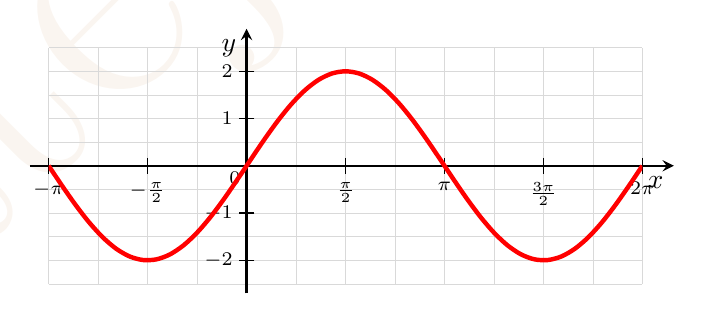
\begin{tikzpicture}[xscale=0.8,yscale=0.6,>=stealth]
\draw[very thin,gray!30,xstep=0.785398,ystep=0.5] (-3.1416,-2.5) grid (6.2832,2.5);
\draw[->,thick] (-3.4416,0) -- (6.7832,0) node[below left] {$x$};
\draw[->,thick] (0,-2.7) -- (0,2.9) node[below left] {$y$};
\draw (-3.1416,0.1667) -- (-3.1416,-0.1667);
\node[below,inner sep=2pt] at (-3.1416,-0.2167) {\scriptsize $-\pi$};
\draw (-1.5708,0.1667) -- (-1.5708,-0.1667);
\node[below,inner sep=2pt] at (-1.5708,-0.2167) {\scriptsize $-\tfrac{\pi}{2}$};
\draw (1.5708,0.1667) -- (1.5708,-0.1667);
\node[below,inner sep=2pt] at (1.5708,-0.2167) {\scriptsize $\tfrac{\pi}{2}$};
\draw (3.1416,0.1667) -- (3.1416,-0.1667);
\node[below,inner sep=2pt] at (3.1416,-0.2167) {\scriptsize $\pi$};
\draw (4.7124,0.1667) -- (4.7124,-0.1667);
\node[below,inner sep=2pt] at (4.7124,-0.2167) {\scriptsize $\tfrac{3\pi}{2}$};
\draw (6.2832,0.1667) -- (6.2832,-0.1667);
\node[below,inner sep=2pt] at (6.2832,-0.2167) {\scriptsize $2\pi$};
\draw (0.1250,-2) -- (-0.1250,-2) node[left,inner sep=2pt] {\scriptsize $-2$};
\draw (0.1250,-1) -- (-0.1250,-1) node[left,inner sep=2pt] {\scriptsize $-1$};
\draw (0.1250,1) -- (-0.1250,1) node[left,inner sep=2pt] {\scriptsize $1$};
\draw (0.1250,2) -- (-0.1250,2) node[left,inner sep=2pt] {\scriptsize $2$};
\node[below left,inner sep=2pt] at (0,0) {\scriptsize $0$};
\begin{scope}
\clip (-3.1416,-2.5) rectangle (6.2832,2.5);
\draw[red,line width=1.6pt,domain=-3.1416:6.2832,samples=45,smooth] plot (\x,{2*sin(deg(\x))});
\end{scope}
\end{tikzpicture}
\end{center}
\item $\displaystyle f(x)=\cos 2x$ \quad ($A=1,\ \omega=\pi,\ Z_f=[-1,1]$)
\begin{center}
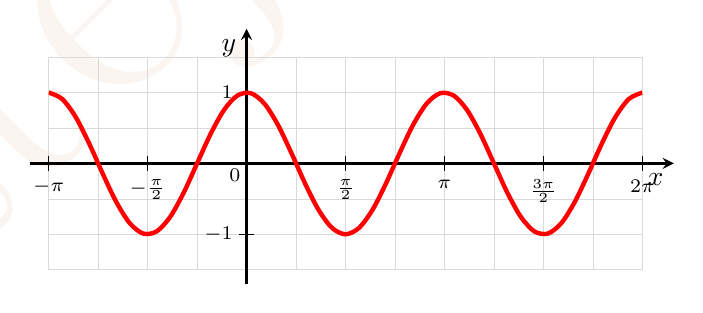
\begin{tikzpicture}[xscale=0.8,yscale=0.9,>=stealth]
\draw[very thin,gray!30,xstep=0.785398,ystep=0.5] (-3.1416,-1.5) grid (6.2832,1.5);
\draw[->,thick] (-3.4416,0) -- (6.7832,0) node[below left] {$x$};
\draw[->,thick] (0,-1.7) -- (0,1.9) node[below left] {$y$};
\draw (-3.1416,0.1111) -- (-3.1416,-0.1111);
\node[below,inner sep=2pt] at (-3.1416,-0.1444) {\scriptsize $-\pi$};
\draw (-1.5708,0.1111) -- (-1.5708,-0.1111);
\node[below,inner sep=2pt] at (-1.5708,-0.1444) {\scriptsize $-\tfrac{\pi}{2}$};
\draw (1.5708,0.1111) -- (1.5708,-0.1111);
\node[below,inner sep=2pt] at (1.5708,-0.1444) {\scriptsize $\tfrac{\pi}{2}$};
\draw (3.1416,0.1111) -- (3.1416,-0.1111);
\node[below,inner sep=2pt] at (3.1416,-0.1444) {\scriptsize $\pi$};
\draw (4.7124,0.1111) -- (4.7124,-0.1111);
\node[below,inner sep=2pt] at (4.7124,-0.1444) {\scriptsize $\tfrac{3\pi}{2}$};
\draw (6.2832,0.1111) -- (6.2832,-0.1111);
\node[below,inner sep=2pt] at (6.2832,-0.1444) {\scriptsize $2\pi$};
\draw (0.1250,-1) -- (-0.1250,-1) node[left,inner sep=2pt] {\scriptsize $-1$};
\draw (0.1250,1) -- (-0.1250,1) node[left,inner sep=2pt] {\scriptsize $1$};
\node[below left,inner sep=2pt] at (0,0) {\scriptsize $0$};
\begin{scope}
\clip (-3.1416,-1.5) rectangle (6.2832,1.5);
\draw[red,line width=1.6pt,domain=-3.1416:6.2832,samples=45,smooth] plot (\x,{cos(deg(2*\x))});
\end{scope}
\end{tikzpicture}
\end{center}
\item $\displaystyle f(x)=\sin\big(x-\tfrac{\pi}{4}\big)$ \quad ($\text{premik za }\tfrac{\pi}{4}\text{ desno},\ \omega=2\pi,\ Z_f=[-1,1]$)
\begin{center}
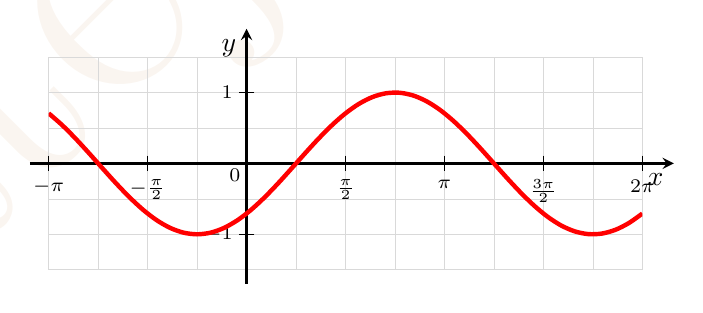
\begin{tikzpicture}[xscale=0.8,yscale=0.9,>=stealth]
\draw[very thin,gray!30,xstep=0.785398,ystep=0.5] (-3.1416,-1.5) grid (6.2832,1.5);
\draw[->,thick] (-3.4416,0) -- (6.7832,0) node[below left] {$x$};
\draw[->,thick] (0,-1.7) -- (0,1.9) node[below left] {$y$};
\draw (-3.1416,0.1111) -- (-3.1416,-0.1111);
\node[below,inner sep=2pt] at (-3.1416,-0.1444) {\scriptsize $-\pi$};
\draw (-1.5708,0.1111) -- (-1.5708,-0.1111);
\node[below,inner sep=2pt] at (-1.5708,-0.1444) {\scriptsize $-\tfrac{\pi}{2}$};
\draw (1.5708,0.1111) -- (1.5708,-0.1111);
\node[below,inner sep=2pt] at (1.5708,-0.1444) {\scriptsize $\tfrac{\pi}{2}$};
\draw (3.1416,0.1111) -- (3.1416,-0.1111);
\node[below,inner sep=2pt] at (3.1416,-0.1444) {\scriptsize $\pi$};
\draw (4.7124,0.1111) -- (4.7124,-0.1111);
\node[below,inner sep=2pt] at (4.7124,-0.1444) {\scriptsize $\tfrac{3\pi}{2}$};
\draw (6.2832,0.1111) -- (6.2832,-0.1111);
\node[below,inner sep=2pt] at (6.2832,-0.1444) {\scriptsize $2\pi$};
\draw (0.1250,-1) -- (-0.1250,-1) node[left,inner sep=2pt] {\scriptsize $-1$};
\draw (0.1250,1) -- (-0.1250,1) node[left,inner sep=2pt] {\scriptsize $1$};
\node[below left,inner sep=2pt] at (0,0) {\scriptsize $0$};
\begin{scope}
\clip (-3.1416,-1.5) rectangle (6.2832,1.5);
\draw[red,line width=1.6pt,domain=-3.1416:6.2832,samples=45,smooth] plot (\x,{sin(deg(\x-pi/4))});
\end{scope}
\end{tikzpicture}
\end{center}
\item $\displaystyle f(x)=-3\cos x$ \quad ($A=3,\ \text{zrcaljenje \v{c}ez os }x,\ \omega=2\pi,\ Z_f=[-3,3]$)
\begin{center}
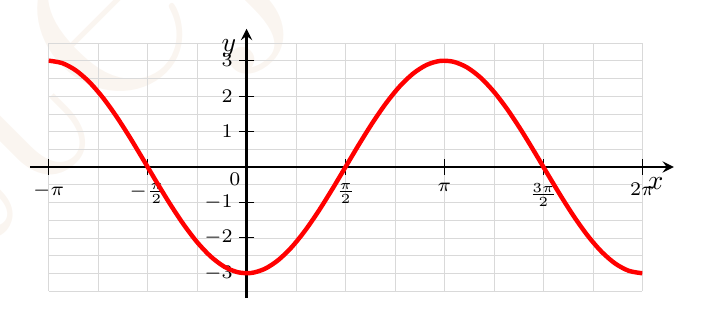
\begin{tikzpicture}[xscale=0.8,yscale=0.45,>=stealth]
\draw[very thin,gray!30,xstep=0.785398,ystep=0.5] (-3.1416,-3.5) grid (6.2832,3.5);
\draw[->,thick] (-3.4416,0) -- (6.7832,0) node[below left] {$x$};
\draw[->,thick] (0,-3.7) -- (0,3.9) node[below left] {$y$};
\draw (-3.1416,0.2222) -- (-3.1416,-0.2222);
\node[below,inner sep=2pt] at (-3.1416,-0.2889) {\scriptsize $-\pi$};
\draw (-1.5708,0.2222) -- (-1.5708,-0.2222);
\node[below,inner sep=2pt] at (-1.5708,-0.2889) {\scriptsize $-\tfrac{\pi}{2}$};
\draw (1.5708,0.2222) -- (1.5708,-0.2222);
\node[below,inner sep=2pt] at (1.5708,-0.2889) {\scriptsize $\tfrac{\pi}{2}$};
\draw (3.1416,0.2222) -- (3.1416,-0.2222);
\node[below,inner sep=2pt] at (3.1416,-0.2889) {\scriptsize $\pi$};
\draw (4.7124,0.2222) -- (4.7124,-0.2222);
\node[below,inner sep=2pt] at (4.7124,-0.2889) {\scriptsize $\tfrac{3\pi}{2}$};
\draw (6.2832,0.2222) -- (6.2832,-0.2222);
\node[below,inner sep=2pt] at (6.2832,-0.2889) {\scriptsize $2\pi$};
\draw (0.1250,-3) -- (-0.1250,-3) node[left,inner sep=2pt] {\scriptsize $-3$};
\draw (0.1250,-2) -- (-0.1250,-2) node[left,inner sep=2pt] {\scriptsize $-2$};
\draw (0.1250,-1) -- (-0.1250,-1) node[left,inner sep=2pt] {\scriptsize $-1$};
\draw (0.1250,1) -- (-0.1250,1) node[left,inner sep=2pt] {\scriptsize $1$};
\draw (0.1250,2) -- (-0.1250,2) node[left,inner sep=2pt] {\scriptsize $2$};
\draw (0.1250,3) -- (-0.1250,3) node[left,inner sep=2pt] {\scriptsize $3$};
\node[below left,inner sep=2pt] at (0,0) {\scriptsize $0$};
\begin{scope}
\clip (-3.1416,-3.5) rectangle (6.2832,3.5);
\draw[red,line width=1.6pt,domain=-3.1416:6.2832,samples=45,smooth] plot (\x,{-3*cos(deg(\x))});
\end{scope}
\end{tikzpicture}
\end{center}
\item $\displaystyle f(x)=2\cos\tfrac{x}{2}+1$ \quad ($A=2,\ \omega=4\pi,\ \text{premik za 1 gor},\ Z_f=[-1,3]$)
\begin{center}
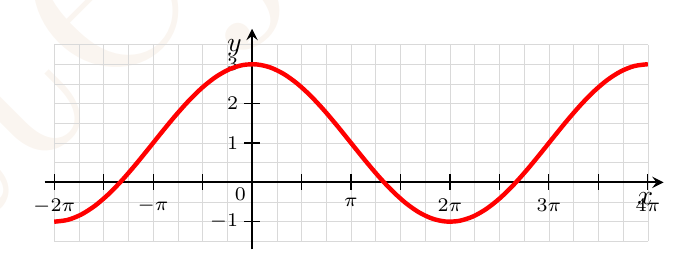
\begin{tikzpicture}[xscale=0.4,yscale=0.5,>=stealth]
\draw[very thin,gray!30,xstep=0.785398,ystep=0.5] (-6.2832,-1.5) grid (12.5664,3.5);
\draw[->,thick] (-6.5832,0) -- (13.0664,0) node[below left] {$x$};
\draw[->,thick] (0,-1.7) -- (0,3.9) node[below left] {$y$};
\draw (-6.2832,0.2000) -- (-6.2832,-0.2000);
\node[below,inner sep=2pt] at (-6.2832,-0.2600) {\scriptsize $-2\pi$};
\draw (-4.7124,0.2000) -- (-4.7124,-0.2000);
\draw (-3.1416,0.2000) -- (-3.1416,-0.2000);
\node[below,inner sep=2pt] at (-3.1416,-0.2600) {\scriptsize $-\pi$};
\draw (-1.5708,0.2000) -- (-1.5708,-0.2000);
\draw (1.5708,0.2000) -- (1.5708,-0.2000);
\draw (3.1416,0.2000) -- (3.1416,-0.2000);
\node[below,inner sep=2pt] at (3.1416,-0.2600) {\scriptsize $\pi$};
\draw (4.7124,0.2000) -- (4.7124,-0.2000);
\draw (6.2832,0.2000) -- (6.2832,-0.2000);
\node[below,inner sep=2pt] at (6.2832,-0.2600) {\scriptsize $2\pi$};
\draw (7.8540,0.2000) -- (7.8540,-0.2000);
\draw (9.4248,0.2000) -- (9.4248,-0.2000);
\node[below,inner sep=2pt] at (9.4248,-0.2600) {\scriptsize $3\pi$};
\draw (10.9956,0.2000) -- (10.9956,-0.2000);
\draw (12.5664,0.2000) -- (12.5664,-0.2000);
\node[below,inner sep=2pt] at (12.5664,-0.2600) {\scriptsize $4\pi$};
\draw (0.2500,-1) -- (-0.2500,-1) node[left,inner sep=2pt] {\scriptsize $-1$};
\draw (0.2500,1) -- (-0.2500,1) node[left,inner sep=2pt] {\scriptsize $1$};
\draw (0.2500,2) -- (-0.2500,2) node[left,inner sep=2pt] {\scriptsize $2$};
\draw (0.2500,3) -- (-0.2500,3) node[left,inner sep=2pt] {\scriptsize $3$};
\node[below left,inner sep=2pt] at (0,0) {\scriptsize $0$};
\begin{scope}
\clip (-6.2832,-1.5) rectangle (12.5664,3.5);
\draw[red,line width=1.6pt,domain=-6.2832:12.5664,samples=45,smooth] plot (\x,{2*cos(deg(\x/2))+1});
\end{scope}
\end{tikzpicture}
\end{center}
\item $\displaystyle f(x)=2\sin 2x-1$ \quad ($A=2,\ \omega=\pi,\ \text{premik za 1 dol},\ Z_f=[-3,1]$)
\begin{center}
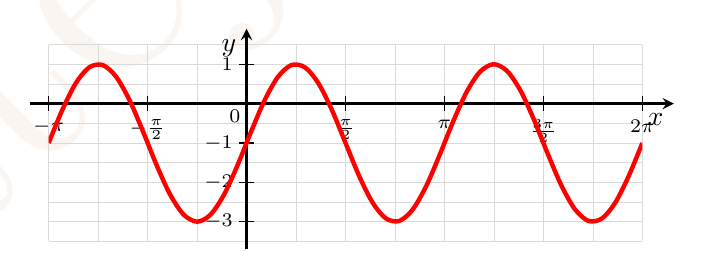
\begin{tikzpicture}[xscale=0.8,yscale=0.5,>=stealth]
\draw[very thin,gray!30,xstep=0.785398,ystep=0.5] (-3.1416,-3.5) grid (6.2832,1.5);
\draw[->,thick] (-3.4416,0) -- (6.7832,0) node[below left] {$x$};
\draw[->,thick] (0,-3.7) -- (0,1.9) node[below left] {$y$};
\draw (-3.1416,0.2000) -- (-3.1416,-0.2000);
\node[below,inner sep=2pt] at (-3.1416,-0.2600) {\scriptsize $-\pi$};
\draw (-1.5708,0.2000) -- (-1.5708,-0.2000);
\node[below,inner sep=2pt] at (-1.5708,-0.2600) {\scriptsize $-\tfrac{\pi}{2}$};
\draw (1.5708,0.2000) -- (1.5708,-0.2000);
\node[below,inner sep=2pt] at (1.5708,-0.2600) {\scriptsize $\tfrac{\pi}{2}$};
\draw (3.1416,0.2000) -- (3.1416,-0.2000);
\node[below,inner sep=2pt] at (3.1416,-0.2600) {\scriptsize $\pi$};
\draw (4.7124,0.2000) -- (4.7124,-0.2000);
\node[below,inner sep=2pt] at (4.7124,-0.2600) {\scriptsize $\tfrac{3\pi}{2}$};
\draw (6.2832,0.2000) -- (6.2832,-0.2000);
\node[below,inner sep=2pt] at (6.2832,-0.2600) {\scriptsize $2\pi$};
\draw (0.1250,-3) -- (-0.1250,-3) node[left,inner sep=2pt] {\scriptsize $-3$};
\draw (0.1250,-2) -- (-0.1250,-2) node[left,inner sep=2pt] {\scriptsize $-2$};
\draw (0.1250,-1) -- (-0.1250,-1) node[left,inner sep=2pt] {\scriptsize $-1$};
\draw (0.1250,1) -- (-0.1250,1) node[left,inner sep=2pt] {\scriptsize $1$};
\node[below left,inner sep=2pt] at (0,0) {\scriptsize $0$};
\begin{scope}
\clip (-3.1416,-3.5) rectangle (6.2832,1.5);
\draw[red,line width=1.6pt,domain=-3.1416:6.2832,samples=45,smooth] plot (\x,{2*sin(deg(2*\x))-1});
\end{scope}
\end{tikzpicture}
\end{center}
\end{enumerate}
\end{resitev}

\begin{resitev}[-- $y=5-10\cos^2x$]
$\displaystyle y=5-10\cdot\frac{1+\cos2x}{2}=-5\cos2x$;\quad $\omega=\pi$,\quad $Z_f=[-5,5]$.\\
Maksimum $y=5$, ko je $\cos2x=-1$: \ $2x=\pi+2k\pi\ \Rightarrow\ \displaystyle x=\frac{\pi}{2}+k\pi,\ k\in\mathbb{Z}$.
\begin{center}
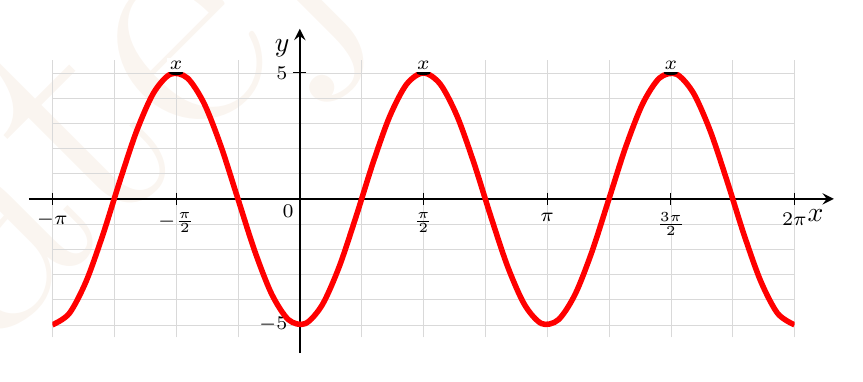
\begin{tikzpicture}[xscale=1,yscale=0.32,>=stealth]
\draw[very thin,gray!30,xstep=0.785398,ystep=1] (-3.1416,-5.5) grid (6.2832,5.5);
\draw[->,thick] (-3.4416,0) -- (6.7832,0) node[below left] {$x$};
\draw[->,thick] (0,-6.125) -- (0,6.75) node[below left] {$y$};
\draw (-3.1416,0.2500) -- (-3.1416,-0.2500);
\node[below,inner sep=2pt] at (-3.1416,-0.3125) {\scriptsize $-\pi$};
\draw (-1.5708,0.2500) -- (-1.5708,-0.2500);
\node[below,inner sep=2pt] at (-1.5708,-0.3125) {\scriptsize $-\tfrac{\pi}{2}$};
\draw (1.5708,0.2500) -- (1.5708,-0.2500);
\node[below,inner sep=2pt] at (1.5708,-0.3125) {\scriptsize $\tfrac{\pi}{2}$};
\draw (3.1416,0.2500) -- (3.1416,-0.2500);
\node[below,inner sep=2pt] at (3.1416,-0.3125) {\scriptsize $\pi$};
\draw (4.7124,0.2500) -- (4.7124,-0.2500);
\node[below,inner sep=2pt] at (4.7124,-0.3125) {\scriptsize $\tfrac{3\pi}{2}$};
\draw (6.2832,0.2500) -- (6.2832,-0.2500);
\node[below,inner sep=2pt] at (6.2832,-0.3125) {\scriptsize $2\pi$};
\draw (0.0800,-5) -- (-0.0800,-5) node[left,inner sep=2pt] {\scriptsize $-5$};
\draw (0.0800,5) -- (-0.0800,5) node[left,inner sep=2pt] {\scriptsize $5$};
\node[below left,inner sep=2pt] at (0,0) {\scriptsize $0$};
\begin{scope}
\clip (-3.1416,-5.5) rectangle (6.2832,5.5);
\draw[red,line width=2pt,domain=-3.1416:6.2832,samples=45,smooth] plot (\x,{5-10*cos(deg(\x))^2});
\end{scope}
\fill[black] (-1.5708,5) circle (2.5pt) node[above,fill=white,inner sep=1pt] {\scriptsize $x$};
\fill[black] (1.5708,5) circle (2.5pt) node[above,fill=white,inner sep=1pt] {\scriptsize $x$};
\fill[black] (4.7124,5) circle (2.5pt) node[above,fill=white,inner sep=1pt] {\scriptsize $x$};
\end{tikzpicture}
\end{center}
\begin{center}\small \tikz[baseline=-0.6ex]\draw[red,line width=2pt] (0,0)--(0.8,0);\ $y=5-10\cos^2x=-5\cos2x$\end{center}

\end{resitev}

\begin{resitev}[-- $y=2-4\sin^2x$]
$\displaystyle y=2-4\cdot\frac{1-\cos2x}{2}=2\cos2x$;\quad $\omega=\pi$,\quad $Z_f=[-2,2]$.\\
Minimum $y=-2$, ko je $\cos2x=-1$: \ $\displaystyle x=\frac{\pi}{2}+k\pi,\ k\in\mathbb{Z}$.
\begin{center}
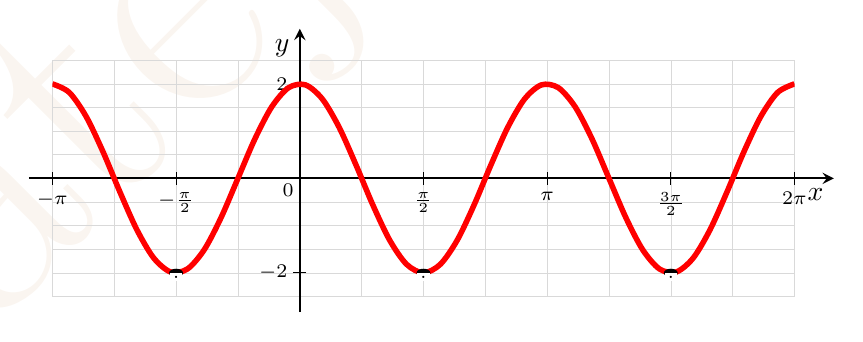
\begin{tikzpicture}[xscale=1,yscale=0.6,>=stealth]
\draw[very thin,gray!30,xstep=0.785398,ystep=0.5] (-3.1416,-2.5) grid (6.2832,2.5);
\draw[->,thick] (-3.4416,0) -- (6.7832,0) node[below left] {$x$};
\draw[->,thick] (0,-2.83333) -- (0,3.16667) node[below left] {$y$};
\draw (-3.1416,0.1333) -- (-3.1416,-0.1333);
\node[below,inner sep=2pt] at (-3.1416,-0.1667) {\scriptsize $-\pi$};
\draw (-1.5708,0.1333) -- (-1.5708,-0.1333);
\node[below,inner sep=2pt] at (-1.5708,-0.1667) {\scriptsize $-\tfrac{\pi}{2}$};
\draw (1.5708,0.1333) -- (1.5708,-0.1333);
\node[below,inner sep=2pt] at (1.5708,-0.1667) {\scriptsize $\tfrac{\pi}{2}$};
\draw (3.1416,0.1333) -- (3.1416,-0.1333);
\node[below,inner sep=2pt] at (3.1416,-0.1667) {\scriptsize $\pi$};
\draw (4.7124,0.1333) -- (4.7124,-0.1333);
\node[below,inner sep=2pt] at (4.7124,-0.1667) {\scriptsize $\tfrac{3\pi}{2}$};
\draw (6.2832,0.1333) -- (6.2832,-0.1333);
\node[below,inner sep=2pt] at (6.2832,-0.1667) {\scriptsize $2\pi$};
\draw (0.0800,-2) -- (-0.0800,-2) node[left,inner sep=2pt] {\scriptsize $-2$};
\draw (0.0800,2) -- (-0.0800,2) node[left,inner sep=2pt] {\scriptsize $2$};
\node[below left,inner sep=2pt] at (0,0) {\scriptsize $0$};
\begin{scope}
\clip (-3.1416,-2.5) rectangle (6.2832,2.5);
\draw[red,line width=2pt,domain=-3.1416:6.2832,samples=45,smooth] plot (\x,{2-4*sin(deg(\x))^2});
\end{scope}
\fill[black] (-1.5708,-2) circle (2.5pt) node[below,fill=white,inner sep=1pt] {\scriptsize $.$};
\fill[black] (1.5708,-2) circle (2.5pt) node[below,fill=white,inner sep=1pt] {\scriptsize $.$};
\fill[black] (4.7124,-2) circle (2.5pt) node[below,fill=white,inner sep=1pt] {\scriptsize $.$};
\end{tikzpicture}
\end{center}
\begin{center}\small \tikz[baseline=-0.6ex]\draw[red,line width=2pt] (0,0)--(0.8,0);\ $y=2-4\sin^2x=2\cos2x$\end{center}

\end{resitev}

\begin{resitev}[-- $y=2\sin2x-2\sqrt3\cos2x$]
$\displaystyle A=\sqrt{2^2+(2\sqrt3)^2}=4$:\quad $\displaystyle y=4\Big(\tfrac12\sin2x-\tfrac{\sqrt3}{2}\cos2x\Big)=4\Big(\sin2x\cos\tfrac{\pi}{3}-\cos2x\sin\tfrac{\pi}{3}\Big)=4\sin\Big(2x-\frac{\pi}{3}\Big)$\\
$\omega=\pi$,\quad $Z_f=[-4,4]$,\quad za\v{c}etna vrednost $y(0)=2\cdot0-2\sqrt3\cdot1=-2\sqrt3$.
\begin{center}
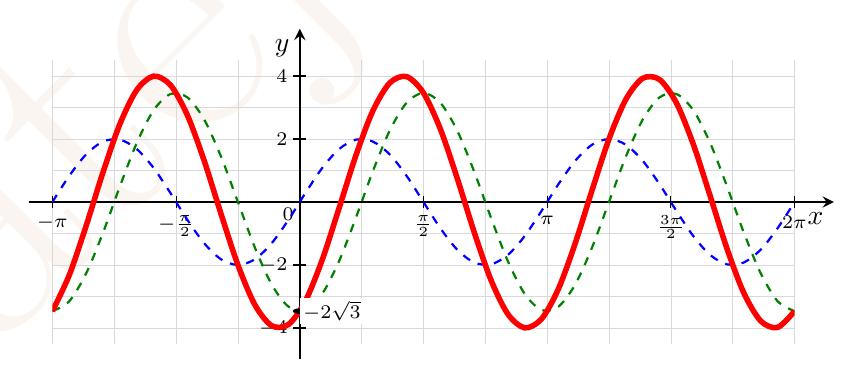
\begin{tikzpicture}[xscale=1,yscale=0.4,>=stealth]
\draw[very thin,gray!30,xstep=0.785398,ystep=1] (-3.1416,-4.5) grid (6.2832,4.5);
\draw[->,thick] (-3.4416,0) -- (6.7832,0) node[below left] {$x$};
\draw[->,thick] (0,-5) -- (0,5.5) node[below left] {$y$};
\draw (-3.1416,0.2000) -- (-3.1416,-0.2000);
\node[below,inner sep=2pt] at (-3.1416,-0.2500) {\scriptsize $-\pi$};
\draw (-1.5708,0.2000) -- (-1.5708,-0.2000);
\node[below,inner sep=2pt] at (-1.5708,-0.2500) {\scriptsize $-\tfrac{\pi}{2}$};
\draw (1.5708,0.2000) -- (1.5708,-0.2000);
\node[below,inner sep=2pt] at (1.5708,-0.2500) {\scriptsize $\tfrac{\pi}{2}$};
\draw (3.1416,0.2000) -- (3.1416,-0.2000);
\node[below,inner sep=2pt] at (3.1416,-0.2500) {\scriptsize $\pi$};
\draw (4.7124,0.2000) -- (4.7124,-0.2000);
\node[below,inner sep=2pt] at (4.7124,-0.2500) {\scriptsize $\tfrac{3\pi}{2}$};
\draw (6.2832,0.2000) -- (6.2832,-0.2000);
\node[below,inner sep=2pt] at (6.2832,-0.2500) {\scriptsize $2\pi$};
\draw (0.0800,-4) -- (-0.0800,-4) node[left,inner sep=2pt] {\scriptsize $-4$};
\draw (0.0800,-2) -- (-0.0800,-2) node[left,inner sep=2pt] {\scriptsize $-2$};
\draw (0.0800,2) -- (-0.0800,2) node[left,inner sep=2pt] {\scriptsize $2$};
\draw (0.0800,4) -- (-0.0800,4) node[left,inner sep=2pt] {\scriptsize $4$};
\node[below left,inner sep=2pt] at (0,0) {\scriptsize $0$};
\begin{scope}
\clip (-3.1416,-4.5) rectangle (6.2832,4.5);
\draw[blue,dashed,thick,domain=-3.1416:6.2832,samples=45,smooth] plot (\x,{2*sin(deg(2*\x))});
\draw[green!50!black,dashed,thick,domain=-3.1416:6.2832,samples=45,smooth] plot (\x,{-2*sqrt(3)*cos(deg(2*\x))});
\draw[red,line width=2pt,domain=-3.1416:6.2832,samples=45,smooth] plot (\x,{4*sin(deg(2*\x-pi/3))});
\end{scope}
\fill[black] (0,-3.4641) circle (2.5pt) node[right,fill=white,inner sep=1pt] {\scriptsize $-2\sqrt3$};
\end{tikzpicture}
\end{center}
\begin{center}\small \tikz[baseline=-0.6ex]\draw[blue,dashed,thick] (0,0)--(0.8,0);\ $y=2\sin2x$ \quad \tikz[baseline=-0.6ex]\draw[green!50!black,dashed,thick] (0,0)--(0.8,0);\ $y=-2\sqrt3\cos2x$ \quad \tikz[baseline=-0.6ex]\draw[red,line width=2pt] (0,0)--(0.8,0);\ $y=4\sin\big(2x-\tfrac{\pi}{3}\big)$\end{center}

\end{resitev}

\begin{resitev}[-- $y=\sqrt3\cos2x-\sin2x$]
$\displaystyle A=\sqrt{(\sqrt3)^2+1^2}=2$:\quad $\displaystyle y=2\Big(\tfrac{\sqrt3}{2}\cos2x-\tfrac12\sin2x\Big)=2\Big(\cos2x\cos\tfrac{\pi}{6}-\sin2x\sin\tfrac{\pi}{6}\Big)=2\cos\Big(2x+\frac{\pi}{6}\Big)$\\
$\omega=\pi$,\quad $Z_f=[-2,2]$,\quad za\v{c}etna vrednost $y(0)=\sqrt3\cdot1-0=\sqrt3$.
\begin{center}
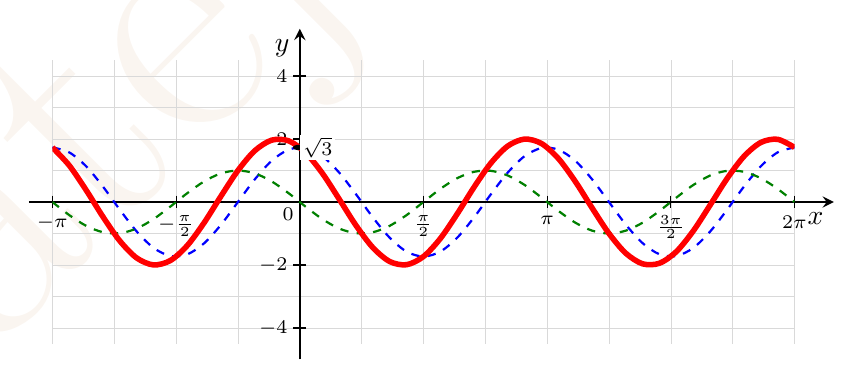
\begin{tikzpicture}[xscale=1,yscale=0.4,>=stealth]
\draw[very thin,gray!30,xstep=0.785398,ystep=1] (-3.1416,-4.5) grid (6.2832,4.5);
\draw[->,thick] (-3.4416,0) -- (6.7832,0) node[below left] {$x$};
\draw[->,thick] (0,-5) -- (0,5.5) node[below left] {$y$};
\draw (-3.1416,0.2000) -- (-3.1416,-0.2000);
\node[below,inner sep=2pt] at (-3.1416,-0.2500) {\scriptsize $-\pi$};
\draw (-1.5708,0.2000) -- (-1.5708,-0.2000);
\node[below,inner sep=2pt] at (-1.5708,-0.2500) {\scriptsize $-\tfrac{\pi}{2}$};
\draw (1.5708,0.2000) -- (1.5708,-0.2000);
\node[below,inner sep=2pt] at (1.5708,-0.2500) {\scriptsize $\tfrac{\pi}{2}$};
\draw (3.1416,0.2000) -- (3.1416,-0.2000);
\node[below,inner sep=2pt] at (3.1416,-0.2500) {\scriptsize $\pi$};
\draw (4.7124,0.2000) -- (4.7124,-0.2000);
\node[below,inner sep=2pt] at (4.7124,-0.2500) {\scriptsize $\tfrac{3\pi}{2}$};
\draw (6.2832,0.2000) -- (6.2832,-0.2000);
\node[below,inner sep=2pt] at (6.2832,-0.2500) {\scriptsize $2\pi$};
\draw (0.0800,-4) -- (-0.0800,-4) node[left,inner sep=2pt] {\scriptsize $-4$};
\draw (0.0800,-2) -- (-0.0800,-2) node[left,inner sep=2pt] {\scriptsize $-2$};
\draw (0.0800,2) -- (-0.0800,2) node[left,inner sep=2pt] {\scriptsize $2$};
\draw (0.0800,4) -- (-0.0800,4) node[left,inner sep=2pt] {\scriptsize $4$};
\node[below left,inner sep=2pt] at (0,0) {\scriptsize $0$};
\begin{scope}
\clip (-3.1416,-4.5) rectangle (6.2832,4.5);
\draw[blue,dashed,thick,domain=-3.1416:6.2832,samples=45,smooth] plot (\x,{sqrt(3)*cos(deg(2*\x))});
\draw[green!50!black,dashed,thick,domain=-3.1416:6.2832,samples=45,smooth] plot (\x,{-sin(deg(2*\x))});
\draw[red,line width=2pt,domain=-3.1416:6.2832,samples=45,smooth] plot (\x,{2*cos(deg(2*\x+pi/6))});
\end{scope}
\fill[black] (0,1.7321) circle (2.5pt) node[right,fill=white,inner sep=1pt] {\scriptsize $\sqrt3$};
\end{tikzpicture}
\end{center}
\begin{center}\small \tikz[baseline=-0.6ex]\draw[blue,dashed,thick] (0,0)--(0.8,0);\ $y=\sqrt3\cos2x$ \quad \tikz[baseline=-0.6ex]\draw[green!50!black,dashed,thick] (0,0)--(0.8,0);\ $y=-\sin2x$ \quad \tikz[baseline=-0.6ex]\draw[red,line width=2pt] (0,0)--(0.8,0);\ $y=2\cos\big(2x+\tfrac{\pi}{6}\big)$\end{center}

\end{resitev}

\end{document}